\chapter{Representing Information for GDPR Compliance using Ontologies}
\label{chapter:vocabularies}

This chapter presents the ontologies developed to fulfil research objective $RO3$ defined in \autoref{sec:intro:RO} regarding creating OWL2 ontologies for representation of information.
It first expands on the methodology in \autoref{sec:intro:ontology-engineering} for developing and evaluating the ontologies based on the summary presented in \autoref{sec:voc:methodology}.
It then presents the developed ontologies which consist of - (i) GDPRtEXT (\autoref{sec:voc:GDPRtEXT}) which provides a linked data representation of GDPR text and a glossary of GDPR compliance concepts, and which satisfies research objective $RO3(a)$ by providing an ontological representation of concepts and text of the GDPR; (ii) GDPRov \autoref{sec:voc:GDPRov} which enables representing provenance of activities associated with personal data and consent in ex-ante and ex-post phases, and fulfils research objective $RO3(b)$ regarding ontological representation of activities associated with processing of personal data and consent; and (iii) GConsent (\autoref{sec:voc:GConsent}) which enables representing information regarding consent, and fulfils research objective $RO3(c)$ regarding ontological representation of consent relevant in determination of GDPR compliance.
Each ontology is presented with a summary of its motivation, engineering process, and dissemination. The ontologies are presented with their evaluation based on the extent to which they satisfy the compliance questions presented in \autoref{sec:info:compliance-questions} and based on comparison with relevant approaches in the state of the art following the analysis presented in \autoref{sec:sota:analysis}.

In addition to these, Data Privacy Vocabulary (DPV), initially presented in \autoref{sec:intro:dpvcg}, is also included as an external contribution based on work done by the author within the W3C Data Protection Vocabularies and Controls Community Group (DPVCG), and the overlap of this work with the research presented. \autoref{sec:voc:DPV} presents an overview of the DPV and compares it with the GDPRtEXT, GDPRov, and GConsent ontologies, and demonstrates their similarity in representing information while drawing attention to the distinguishing features.
The section also presents a comparison of DPV with the state of the art as identified in \autoref{chapter:sota}.

\section{Methodology for Ontology Engineering}\label{sec:voc:methodology}

\subsection{Utilisation of Existing Ontology Engineering Methodologies}
The creation of ontologies followed guidelines and methodologies deemed `best practice' by the semantic web community. In this, `Ontology development 101: A guide to creating your first ontology' by Noy and McGuiness \cite{noy_ontology_2001} was utilised as the guiding document for ontology creation. It provided steps for construction of an ontology with attention on avoiding bad design decisions and common pitfalls. It also suggested the use of competency questions to determine the scope of an ontology and for evaluation after creation.
% For this, the compliance questions presented in \autoref{} were used as competency questions.
The guide suggests Protégé\footnote{\url{https://protege.stanford.edu/}} - a popular and widely adopted tool - for ontology development as it supports semantic reasoners to detect logical inconsistencies arising from asserted facts and axioms in the ontology.
Use of the guide provided a foundational basis for initiating the ontology development process and for using the compliance questions from \autoref{sec:info:compliance-questions} as competency questions to identify concepts and relationships, testing for inconsistencies using Protégé, and iteratively combining to create an ontology. 

The development of ontologies followed a combination of the NeOn methodology \cite{suarez-figueroa_neon_2012} and UPON Lite methodology \cite{de_nicola_lightweight_2016}. NeOn provides a flexible workflow through the use of scenarios which can be adapted for ontology development. The scenarios include implementing using a specification, reusing and re-engineering existing ontological and non-ontological resources, and utilisation of ontological design patterns. 
UPON Lite is a lightweight methodology for rapid ontology engineering that was used in combination with NeOn for iteratively developing the presented ontologies. It consists of six steps from identification of domain terminology, construction of domain glossary, creating a taxonomy, predication as properties, meronymy for complex components, and conceptualisation into an ontology.
The combination of the two consisted of identifying the development scenario from NeOn for gathering requirements, and using UPON Lite to derive actionable tasks for ontology creation.

The methodology used to develop the ontologies presented in this chapter explicitly specifies the competency questions used to derive its concepts based on the compliance questions from the previous chapter. This approach enables tracing the lineage of a concept to its role in the compliance process and provides transparency in the development process.
To compare the methodology described with other methodologies used to develop ontologies within the relevant approaches presented in the SotA, some utilise legal experts which act as domain experts to validate the developed ontologies and their interpretation - such as in the research projects SPECIAL and MIREL (see \autoref{sec:sota:gdpr-semweb}). Such projects involve commercial partners who provide real-world use-cases and data to inform and evaluate the developed research.
Others - such as Ujcich et al. \cite{belhajjame_provenance_2018} - interpret the GDPR as a set of requirements for compliance in their modelling of information. In either case, the SotA does not provide competency questions that could be used to develop ontologies\footnote{Deliverables of research project provide a description of how the concepts of their ontologies were developed from legal requirements, but such descriptions are argumentative and limited to the specified domain or use-case, and hence do not provide a concrete requirement that can be used to develop an ontology to answer the compliance questions.}.

% The aims and motivations of this thesis (see \autoref{sec:intro:background}) are based on representing information for assisting the compliance process rather than an evaluation of compliance itself. Therefore, the research has been documented methodologically to indicate its aims, motivations, methodology, and resources used to shape conceptualisations and rationalisations, and published in an open and accessible manner to enable transparency and reuse.

\subsection{Ontology Quality}
The quality of an ontology refers to the quality of its design of concepts and relationships, and quality as a semantic dataset. While following a suitable ontology engineering methodology provides a structured ontology, it still needs to be inspected for quality in terms of ontology as well as for intended use-cases and scenarios. For this, existing publications \cite{gurk_towards_2017,vrandecic_ontology_2010} list various methods of ontology quality detection, evaluation, and suggest solutions to fix identified problems.

OOPS!\footnote{\url{http://oops.linkeddata.es/}} \cite{poveda-villalon_oops!_2014} is a useful tool for ontology evaluation which detects common pitfalls in the design of concepts and relationships and provides a documented output which can be persisted for provenance of ontology development. Each pitfall detected by OOPS! is categorised along  structural, functional, and usability-profiling dimensions. The tool also provides an indicative measure of importance regarding the pitfall in terms of critical, important, and minor levels.
OOPS! was used for detecting catalogued common pitfalls in the periodic evaluation of developed ontologies. Identified pitfalls were corrected by changing the underlying relationships and iteratively developing the ontology to remove them. 

Quality was also assessed and maintained by asserting the sufficiency of developed ontology to represent and query based on collected use-cases presented in \autoref{sec:info:use-cases}. Where the ontology was found deficient in concepts and relationships, these were added in the next iteration. Where existing models were found to be insufficient or incorrect, these were rectified by either removing the offending parts or re-designing them - based on its impact on compatibility with previous versions.

\subsection{Ontology Documentation}
Ontology documentation was created by using the WIDOCO\footnote{\url{https://dgarijo.github.io/Widoco/}} \cite{garijo_widoco_2017} tool which uses ontology metadata to create HTML documents listing its classes and properties. Ontology metadata consists of information regarding the ontology as well as its concepts and properties integrated into the serialisation as annotations. WIDOCO provides a document of suggested metadata indicating best practices for ontology documentation, which the developed ontologies utilised. It builds upon the LODE\footnote{\url{http://www.essepuntato.it/lode}} tool which is itself a popular ontology documentation service.

The output of the WIDOCO tool is a HTML document along with various serialisations of the ontology for content negotiation which can be published and used as an online resource. Additional information was manually added to the HTML documentation regarding aims and methodologies used in the development of ontologies as well as examples of use-cases and diagrams intended for human consumption. WIDOCO integrates OOPS! to detect pitfalls in the ontology and documents the output. It also provides an interactive visualisation of the ontology using WebVOWL\footnote{\url{http://vowl.visualdataweb.org/webvowl.html}}.

\subsection{Dissemination}
The ontologies were published on the internet using a stable IRI through persistent identifiers on servers hosted by ADAPT Research Centre\footnote{\url{https://adaptcentre.ie/}} and School of Computer Science \& Statistics\footnote{\url{https://scss.tcd.ie/}} within Trinity College Dublin. Initially, these were provided through the purl\footnote{\url{https://purl.org/}} service, which later had issues regarding maintenance and frequent problems with URL resolution. The ontologies were then re-engineered to utilise the W3ID\footnote{\url{w3id.org/}} persistent identifiers maintained by the W3C Permanent Identifier Community Group\footnote{\url{https://www.w3.org/community/perma-id/}}. The ontologies published in this manner followed the best practices and principles related to use of Linked Open Data\footnote{\url{https://www.w3.org/TR/ld-bp/}}, Linked Open Vocabularies\footnote{\url{https://dgarijo.github.io/Widoco/doc/bestPractices/index-en.html}}, and FAIR\footnote{Findability, Accessibility, Interoperability, and Reusability (FAIR) \url{https://doi.org/10.1038\%2Fsdata.2016.18}} principles.

Each ontology was added to the Linked Open Vocabularies\footnote{\url{https://lov.linkeddata.es/}} (LOV) community listing which catalogues vocabularies in the semantic web community. Each ontology was published in Zenodo\footnote{\url{zenodo.org/}} which provides open repositories and assigns a unique DOI for the repository and each of its iterations. The ontology development and resources were also added to public hosting services such as GitHub\footnote{\url{github.com/}} and an instance of OpenGogs\footnote{\url{opengogs.adaptcentre.ie/}} hosted on institution servers. Each ontology was published under an open and permissive license (CC-by-4.0\footnote{\url{https://creativecommons.org/licenses/by/4.0/}}) to promote its use and adoption.

\subsection{Evaluation}
Evaluation was carried out by analysing the sufficiency of each ontology to represent information for answering the competency questions. This was carried out in an iterative manner where each iteration consisted of developing the ontology, evaluating it, and utilising the results of evaluation as feedback in identifying areas of improvement for the next iterations such as missing concepts and relationships, or incorrect assumptions expressed in existing ones. Outcomes of this process are presented in the evaluation section of each ontology.

The ontology was also evaluated against common pitfalls using the OOPS! service as described earlier regarding ontology quality. The OOPS! ontology report is published alongside the ontology documentation, and can also be manually generated by using the online service. Documentation and publishing standards were evaluated by assessing whether the ontologies met existing criteria advocated by the community (such as 5-star principle for linked data \footnote{\url{https://5stardata.info/en/}} and the FAIR principles). Finally, each ontology was published and presented in a peer-reviewed venue and publication, with more information provided in the ontology's section.

Evaluation of the work as a research contribution was carried out based on whether it satisfied the research objectives which motivated its development and whether it provided novel contributions compared to the existing approaches within the state of the art. The details of this are presented in the evaluation section of each ontology.

\subsection*{Summary of Methodology}
Based on the above description of ontology engineering processes, the methodology used for ontology engineering and development is summarised through the following steps:
\begin{enumerate}
    \item \textbf{Identification of aims, objectives, scope:} The first step was to identify the aim and objectives of information to be represented, followed by deciding on the scope regarding relation to GDPR compliance. For the ontologies presented in this chapter, the aims and objectives are listed in \autoref{sec:intro:RQ}. % introduction
    \item \textbf{Identify and analyse relevant information:} Using the scope, relevant information was gathered from various sources - including authoritative, community, and publications - and analysed to identify terms of importance and requirements regarding GDPR compliance. The information is presented as background of the GDPR in \autoref{sec:background:GDPR} and analysed with regards to compliance in \autoref{chapter:information}.
    \item \textbf{Create use-cases and competency questions:} From the analysed information, different use-cases were identified to better understand the application of information in compliance scenarios and the requirements of different stakeholders in this process. This was done using the information interoperability model presented in \autoref{sec:info:model}. The analysed information was used to create compliance questions, as presented in \autoref{sec:info:compliance-questions}, which identify relevant information for evaluation of compliance. These compliance questions were utilised as competency questions in the development and evaluation of ontologies.
    \item \textbf{Identify concepts and relationships:} Relevant concepts and relationships were identified to express information required to answer compliance questions in identified use-cases. This was an iterative and cyclic process where identified concepts and relationships were re-purposed to better suit some design pattern or compliance requirements.
    \item \textbf{Create Ontology:} The identified concepts and relationships were formalised as an ontology in OWL2 using the Protégé ontology development environment. In this process, a semantic reasoner (i.e. Pellet\footnote{\url{https://github.com/stardog-union/pellet}} and HermiT\footnote{\url{http://www.hermit-reasoner.com/}}) was used to identify logical inconsistencies in the ontology. Minor inconsistencies were fixed by changing the appropriate relationships between concepts, while major inconsistencies required evaluation of information identified in step 4. Development of the ontology utilised best practices advocated by the semantic web community in terms of ontology metadata, documentation, design patterns, publication, and dissemination.
    \item \textbf{Evaluate:} The ontology was evaluated for sufficiency towards representing information for answering competency questions. The use of a semantic reasoner detected logical inconsistencies in the expressed facts and axioms, while OOPS! provided detection of common pitfalls and bad design patterns.
    The quality of metadata and documentation evaluated in terms of sufficiency based on community guidelines. Where an ontology was published and/or presented as a resource or as part of a peer-reviewed publication, the resulting comments and feedback were used to identify areas of improvement. Citations of the ontologies and associated publications were used to identify criticisms (if provided) and to compare them with work presented in the citing publication.
    \item \textbf{Dissemination:} The ontology and its documentation were published online with a persistent identifier as a FAIR resource with an open and permissive license. This included publication of the ontology, datasets, and code in a public repository accompanied by human-readable documentation about its creation and utilisation.
    \item \textbf{Progressive iterations:} Within a single iteration of development, the ontology was created and evaluated by following steps 2 to 6. Multiple iterations consisted of repeating these steps as in an development cycle to progressively improve the ontology by adding new concepts or removing existing undesirable ones. Previous versions of the ontology were retained with their documentation for provenance where possible.
\end{enumerate}

% \subsection*{Modularity of Ontologies}
% The research question stated in \autoref{sec:intro:RQ} lays the scope for the work of developing an ontological re{}presentation of information associated with GDPR compliance and concerning activities associated with processing of personal data and consent.
% This information is identified through the research objectives $RO1$ and $RO2$.
% They provide the analysis of GDPR and the compliance questions as presented in \autoref{chapter:information} which act as requirements in the ontology engineering process.
% This directly provides the objective of developing an ontology to represent information about processing of personal data and consent.

\section{GDPRtEXT - Linked Open Dataset of GDPR text \& Glossary of Concepts}\label{sec:voc:GDPRtEXT}

This section describes the GDPRtEXT vocabulary and dataset which provides a linked open data version of the text of GDPR and a SKOS glossary of concepts associated with its compliance. The section presents the motivation and creation of GDPRtEXT, its publication and dissemination, and comparison with relevant approaches in the state of the art. GDPRtEXT is available online\footnote{\url{https://w3id.org/GDPRtEXT/}} with its documentation and code repository\footnote{\url{https://github.com/coolharsh55/GDPRtEXT/}}.

\subsection{Motivation}
GDPR as a legislation consists of text which is structured into 173 Recitals, 99 Articles (further grouped into Chapters and Sections), and 21 Citations. Each Article may have one or more Paragraphs, which itself may have one or more Sub-Paragraphs. As is the norm for legislations, each individual clause - whether an article, paragraph, or sub-paragraph - is identified with an alphanumeric number if provided. These are commonly referenced in textual notation by mentioning these identifiers present in the text of the legislation, such as for \textit{Article 8 Paragraph 2 Sub-Paragraph c} the following textual notations can be used: \textit{A8(2-c), A(8-2c), A8-2(c), Art.8 2(c), Art-8-2-c}. As there is no standard or accepted commonality in the approach, and because such notations are intended for human readability and interpretation - a strict set of such notations does not exist. This presents difficulty when representing such information in machine-readable formats.

The EU Publications Office currently publishes legislation metadata at the document level which provides information about GDPR as a legislation using the ELI ontology and standard \cite{thomas_european_2019} but does not specify granular information about its contents - such as its articles. The EU Publications Office has indicated its intention to provide such granular metadata in the future, the state of the art contains primarily two approaches as presented and analysed in \autoref{sota:analysis:representation}. These provide granular information representation of GDPR clauses but are not compatible with the ELI model used by EU Publications Office. Furthermore, the concepts arising from the legislation as well as those used in the context of GDPR compliance have no standardised reference to provide commonality between two representations in different use-cases. 

Within the larger scope of legal compliance, information is always associated with the clauses and concepts of a law - which in this case is the GDPR.
Amongst the approaches part of SotA presented in \autoref{chapter:sota}, only two approaches consider the association of information with GDPR within the scope of their work - as presented in \autoref{sota:analysis:representation}.
The other approaches, if they do model the concepts and clauses of the GDPR, do so in an ad-hoc manner in which references to the GDPR are made in a textual notation such as ``Article 4-11''.
As the analysis in \autoref{sota:analysis:representation} points out, the two approaches modelling clauses of the GDPR have three drawbacks - (a) the representation is incompatible with the ELI ontology used in the publication of the GDPR, (b) none provide a glossary of terms relevant for compliance, and more importantly (c) neither can be reused as it is not published as an open access resource.
The addressing of this gap is therefore also a research objective required to address the research question of this thesis.

With this motivation the research question was established in \autoref{sec:intro:RO} as $RO3(a)$ and is fulfilled by the GDPRtEXT - which provides an OWL2 ontology for granular representation of GDPR text and a dataset created using this ontology for a linked data representation of GDPR. GDPRtEXT also provides a SKOS vocabulary of terms associated with compliance and links them with their definition and use using the developed ontology. Thus, it fulfils the objective of enabling linking of information with individual clauses of the GDPR and with terms related to GDPR compliance.

\subsection{Ontology Engineering and Creation of Resource}\label{sec:voc:gdprtext-engineering}
Following the methodology described in \autoref{sec:voc:methodology}, the development of competency questions was based on the understanding and analysis of how legal articles are referenced in text in relation to compliance. The competency questions are categorised based on whether they concern structure of GDPR or representation of concepts associated with compliance. These competency questions are concerned with associating information with GDPR and thereby differ from the compliance questions presented in \autoref{chapter:information} which are concerned with the evaluation of compliance. The collected competency questions are outlined below with the identified requirements:

\subsubsection{Structure of GDPR text}
\begin{enumerate}[label={\texttt{CQ.\theenumi}}]
    \item How many Recitals are there within GDPR?
    \item How many Chapters are there within GDPR?
    \item How many Sections are there within GDPR?
    \item How many Articles are there within GDPR?
    \item How many Paragraphs are there within GDPR?
    \item How many Sub-paragraphs are there within GDPR?
    \item How many References or Citations are there within GDPR?
    \item Article 4 belongs to which Chapter? (generalised to which \textit{Chapter} does \textit{Article X} belong?)
    \item Which clause contains the definition of 'personal data'? (generalised to definition of \textit{concept X})
    \item What is the structural hierarchy of the document?
    \item What are the `Principles' defined in GDPR? (generalised to \textit{conceptA} with types \textit{conceptB}, e.g. `Accountability' as a type of `Principle')
    \item Which articles, paragraphs, and sub-paragraphs are relevant to the validity of given consent? (generalised to relevant to \textit{concept X})
    \item How to associate information regarding given consent to relevant clauses in the GDPR? (generalised to association information regarding \textit{concept X})
    \item How to associate information regarding compliance to a specific article of the GDPR?
\end{enumerate}

Based on these, the following requirements were identified with regards to extending the existing ELI ontology to represent granular structure:
\begin{itemize}
    \item Structure of text must be specified with granularity and a hierarchy of Document, Chapter, Section, Article, Paragraph, Sub-Paragraph along with Recitals and Citations.
    \item Relations between clauses must be specified e.g. Paragraph belongs to an Article.
    \item Relations must be transitive e.g. Paragraph in an Article must also be in the Article's Chapter.
    \item Each individual clause must have a unique IRI to enable linking of information to it.
\end{itemize}

\subsubsection{Concepts associated with GDPR compliance}
\begin{enumerate}[label={\texttt{CQ.\theenumi}},resume]
    \item What type of data does the GDPR define?
    \item What types of consent does the GDPR define?
    \item What are the different entities referred to within GDPR?
    \item Which activities are associated with processing of personal data?
    \item Which activities are associated with consent?
    \item What are the conditions or criteria associated which affect sensitivity of processing?
    \item What activities are relevant to a data breach?
    \item Which activities are relevant regarding compliance?
    \item What are the principles defined in GDPR?
    \item What are the rights provided by the GDPR?
    \item Which criteria does the GDPR mention for right to data portability?
    \item Which criteria does the GDPR mention for right to be informed?
    \item What are the obligations mentioned within GDPR?
    \item What are the obligations of the Controller?
    \item What are the obligations of the Processor?
    \item What are the obligations of a DPO?
    \item What are the lawful basis for processing of personal data specified in the GDPR?
    \item What are the conditions for valid consent under GDPR?
    \item Which obligations are mentioned in relation to data collection?
    \item Which obligations are mentioned in relation to obtaining consent?
    \item Which obligations are mentioned in relation to retaining personal data?
    \item Which obligations are mentioned in relation to security of personal data?
    \item What concepts are defined regarding seals and certifications?
\end{enumerate}

Based on these, the following requirements were identified with regards to representing concepts using the W3C SKOS standard as a glossary:
\begin{itemize}
    \item The glossary should express concepts in a hierarchy of relation as associated with compliance. This hierarchy is based on which additional concepts are relevant to the given concept. For example, all principles are referred to when referring to the concept of `Principle', and - activities and actions associated with compliance are referred to when using the concept of `Compliance'.
    \item The glossary should reference concepts with their definitions within the clauses of the GDPR.
    \item The glossary should indicate relevant concepts within GDPR for a given concept in the context of compliance.
    \item The glossary should provide concepts regarding:
    \begin{itemize}
        \item types of data
        \item types of consent
        \item types of entities
        \item types of activities associated with - consent, data, processing, data breaches
        \item actions associated with compliance
        \item principles defined in the GDPR
        \item rights provided by the GDPR
        \item obligations mentioned in the GDPR
        \item conditions required for valid consent
        \item conditions associated with seals and certifications
    \end{itemize}
\end{itemize}

\subsubsection{Extending ELI}
The suitability of extending the existing ELI ontology for representing hierarchy of clauses in GDPR was evaluated and found to be feasible based on continued compatibility of concepts. Existing resources associated with the information model used by ELI - namely the FORMEX\footnote{\url{https://op.europa.eu/en/web/eu-vocabularies/formex//}} and Common Data Model\footnote{\url{https://op.europa.eu/en/web/eu-vocabularies/model/-/resource/dataset/cdm}} were used to formulate an extension mechanism that ensured compatibility.
The extension was modelled to be language agnostic with labels in English. Therefore the language specifications provided by FRBR model\footnote{\url{https://www.ifla.org/publications/functional-requirements-for-bibliographic-records}} were not modelled nor included as language labels. This functionality can be integrated in future by extending the data model as per FRBR specifications.

\subsubsection{Creation of datasets}
Three outputs were decided based on the requirements - an OWL2 ontology for representing structure of GDPR text, a dataset of GDPR text using this ontology, and a SKOS glossary of concepts associated with compliance. The OWL2 ontology and SKOS glossary were combined within a single deliverable - namely the GDPRtEXT ontology, and the representation of GDPR text was provided as a RDF dataset with metadata defined using the DCAT\footnote{\url{https://www.w3.org/TR/vocab-dcat/}} and VoID\footnote{\url{https://www.w3.org/TR/void/}} standards.

Extracting the text of GDPR as individual clauses proved to be a challenge due to the way the official legislation is structured and provided in HTML, PDF, and XML serialisations. The task of extracting individual clauses and annotating their structure (e.g. chapter, article, paragraph) was automated using a JavaScript script\footnote{\url{https://github.com/coolharsh55/GDPRtEXT/blob/master/scripts/parse_gdpr.js}}.

Three datasets were produced and published through this process. The first provides description of canonical versions of the official legislation, i.e. published by the EU Publications Office, and describes the GDPR legislation in its HTML, PDF, and XML formats. The second provides a copy of the GDPR text hosted on institution servers and provides identifiers for individual clauses in the GDPR in HTML, JSON, and plain-text formats. The third provides RDF serialisations of the text of GDPR using the GDPRtEXT ontology in RDF/XML, N3, Turtle, and JSON-LD formats.

The glossary published using SKOS utilised the IRIs of individual clauses of the GDPR to indicate source, definitions, and related concepts. Definitions were declared using the \texttt{rdfs:isDefinedBy} property, and a new property called \texttt{gdprtext:involves} was created to indicate associations. 

\subsubsection{Publication \& Dissemination}
The ontology and dataset were made available through a SPARQL end-point\footnote{\url{https://w3id.org/GDPRtEXT/sparql}} on a triple-store hosted on the institution servers. Pubby\footnote{\url{http://wifo5-03.informatik.uni-mannheim.de/pubby/}} was used to provide a front-end for browsing the RDF serialisation of GDPRtEXT, as shown in \autoref{fig:vocab:gdprtext-pubby}. The dataset was provided under the CC-by-4.0 license to provide resources in an open and reusable manner and was published in the Irish Open Data Portal\footnote{\url{https://data.gov.ie/dataset/gdprtext}} which rated it as a 5-star linked open dataset indicating the highest quality rating. \begin{figure}[htbp]
    \centering
    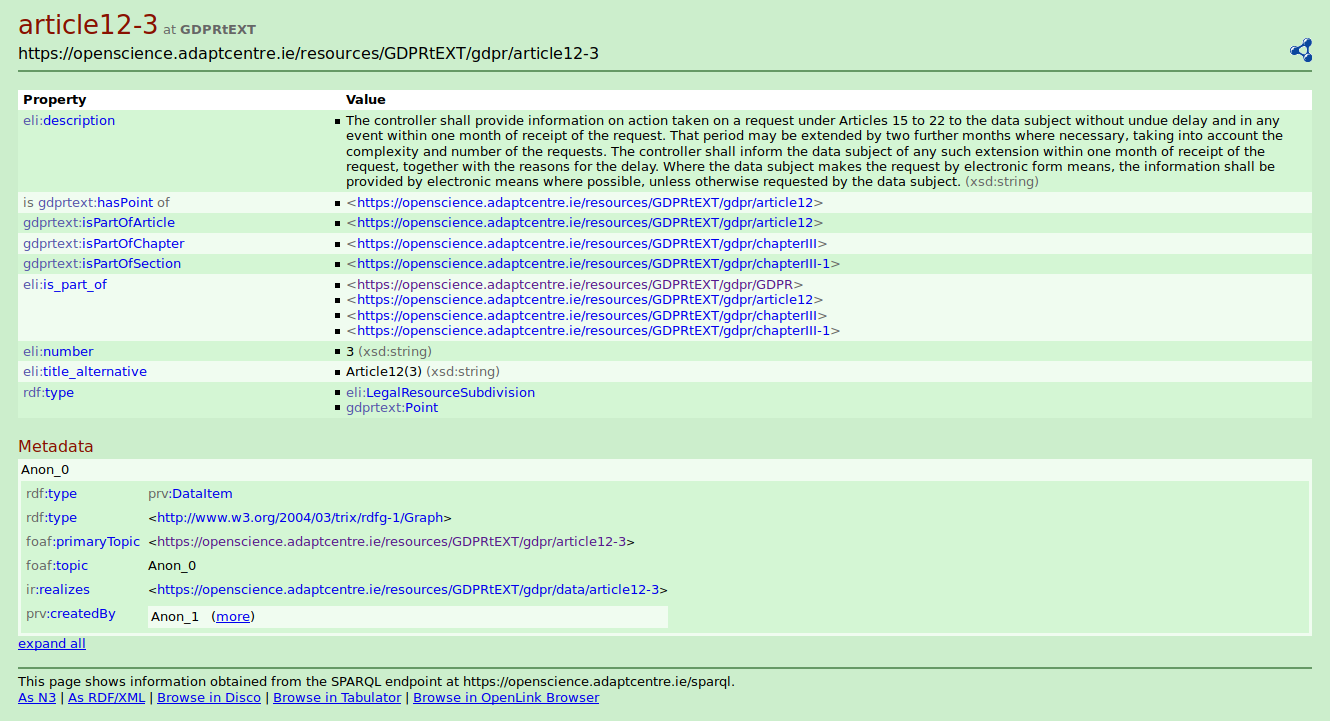
\includegraphics[width=\linewidth]{img/gdprtext-pubby}
    \caption{Article 12(3) in GDPRtEXT as RDF displayed using Pubby \cite{pandit_gdprtext_2018}}
    \label{fig:vocab:gdprtext-pubby}
\end{figure}

\subsection{Resource Description \& Application}
An visual overview of the structuring of concepts within GDPRtEXT is presented in \autoref{fig:vocab:gdprtext-summary-a} and \autoref{fig:vocab:gdprtext-summary-b}.

\begin{figure}[htbp]
    \centering
    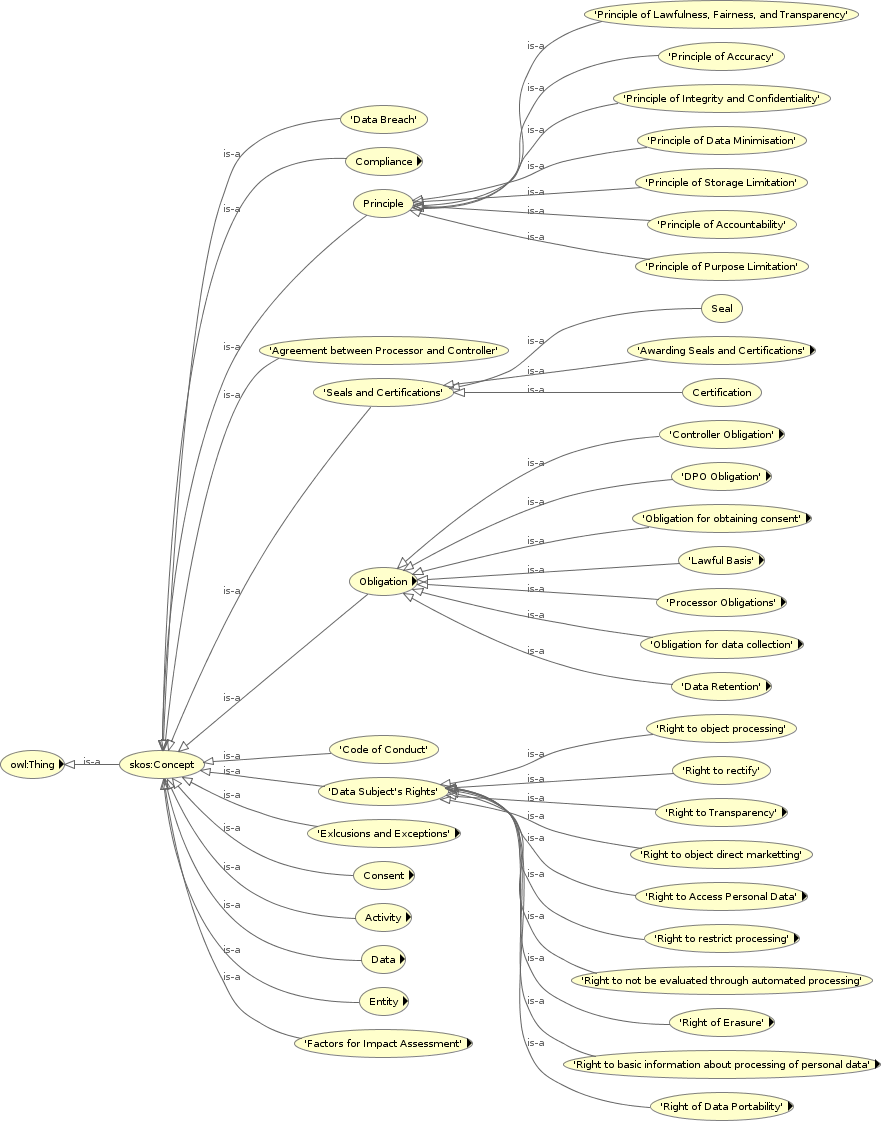
\includegraphics[width=\linewidth]{img/gdprtext-summary-a}
    \caption{Visual overview of concepts in GDPRtEXT - part (a) \cite{pandit_gdprtext_2018}}
    \label{fig:vocab:gdprtext-summary-a}
\end{figure}
\begin{figure}[htbp]
    \centering
    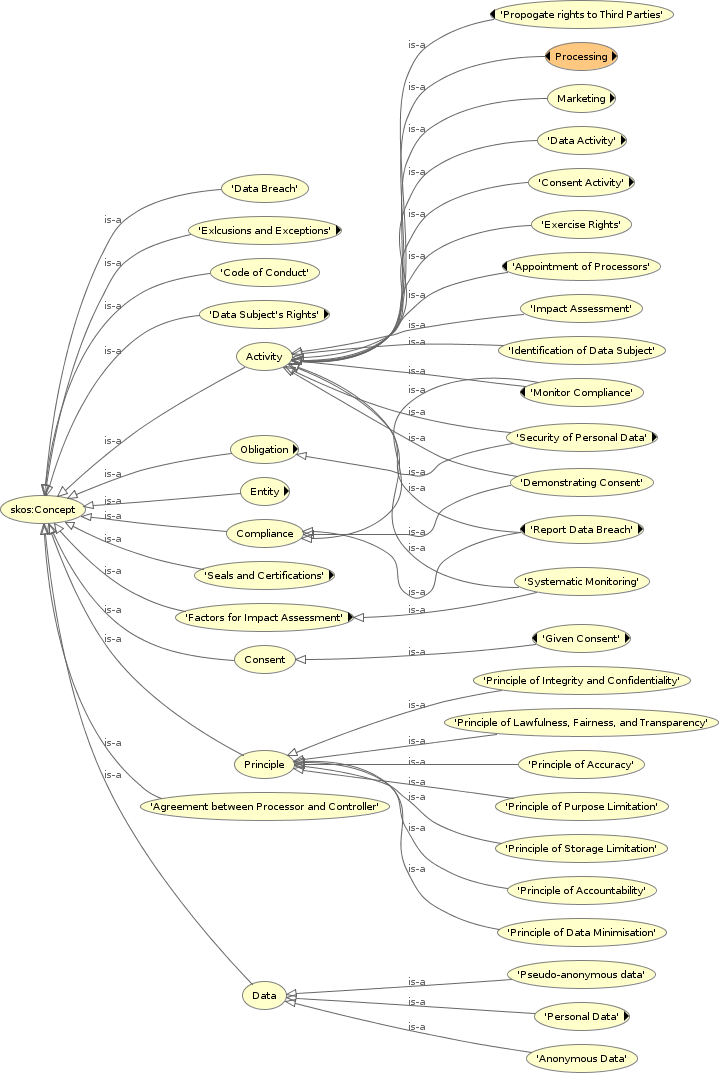
\includegraphics[width=0.75\linewidth]{img/gdprtext-summary-b}
    \caption{Visual overview of concepts in GDPRtEXT - part (b) \cite{pandit_gdprtext_2018}}
    \label{fig:vocab:gdprtext-summary-b}
\end{figure}

\subsubsection{Concepts for description structure of text}
GDPRtEXT extends the European Legislation Identifier (ELI) \cite{thomas_european_2019} ontology published by the European Publications Office with granular concepts to represent each individual clause within the GDPR. 
ELI provides the class \texttt{LegalResource} to indicate a legislative document and its sub-class \texttt{LegalSubResource} to indicate a component or part of that resource. GDPRtEXT extends the \texttt{LegalSubResource} concept with classes \texttt{Chapter}, \texttt{Section}, \texttt{Article}, \texttt{Point} (indicates Paragraph), \texttt{SubPoint} (indicates Sub-Paragraph), \texttt{Recital}, and \texttt{Citation} using the sub-class mechanism.
The ELI ontology provides properties \texttt{has\_part} and its inverse \texttt{is\_part\_of} to indicate connections between two legal resources. GDPRtEXT extends these to indicate hierarchical relations between chapters, sections, articles, points, and sub-points.

\subsubsection{Concepts about Data}
GDPR mentions different types of data, based on which various obligations and requirements are set forth in relation to compliance. GDPRtEXT provides the top-level concept of \texttt{Data} to indicate the abstract term of `data'.
The GDPR primarily focuses on personal data as defined in Article 4(1) - which is represented in GDPRtEXT as \texttt{PersonalData}, with special categories defined in Article 9(1) requiring additional obligations regarding its processing and handling and represented by \texttt{SpecialCategoryPersonalData}. Types of special categories mentioned include criminal data, genetic data, health data, and racial data which are defined as sub-classes in GDPRtEXT.
GDPR also mentions data in the context of anonymisation and pseudo-anonymisation processes, with their outcomes specified using the \texttt{AnonymousData} and \texttt{PseudoAnonymousData} concepts.

\subsubsection{Concepts about Consent}
The top-level concept of `consent' is represented by \texttt{Consent} in GDPRtEXT with its definitions based in Articles 4(11), 6(1) and Recitals 32, 40. It is sub-classed to indicate `given consent' - which is a legal basis and is therefore a sub-class of both \texttt{Consent} and \texttt{LegalBasis}. \texttt{GivenConsent} is further sub-classed to indicate `valid consent' which carries obligations of ensuring the consent is valid and meets the requirements of GDPR and is therefore also defined as the sub-class of \texttt{ObligationForObtainingConsent}. These obligations are represented by sub-classing the \texttt{ValidConsent} concept regarding conditions of - freely given, informed, specific, voluntary, and opt-in.

\subsubsection{Concepts about Entities}
\texttt{Entity} represents the top-level concept of `entity' indicating any institution, company, corporation, partnership, government agency, university, or any other organisation including individuals. 
It is sub-classed to indicate entities mentioned in GDPR, which are - Data Subject, Controller, Processor, Sub-Processor, Data Protection Officer (DPO), and Data Protection Authority (DPA). Additionally, relevant concepts associated with entities are also defined, which are -  Representative of Controller, Representative of Processor, Certification Body, and Regulatory Authority.

\subsubsection{Concepts about Activities}
`Activity' refers to some process or action mentioned, referred, implied, or defined by the requirements of GDPR compliance. To represent these, GDPRtEXT defines activities regarding consent and personal data processing, as well as other activities related to the functioning of the GDPR such as reporting data breach and demonstrating consent. The top-level concept `Activity' represents the abstraction of all activities. `ConsentActivity' and `DataActivity' represent specialised activities representing involvement of consent and personal data respectively.

Consent activities defined within GDPRtEXT consist of obtaining consent and withdrawing consent. Data activities provided include use, archival, collection, cross-border transfer, erasure, copying, rectifying, sharing, and storage of personal data. In these, the activity associated with usage of personal data is equivalent to its common and synonymous usage with the term `processing'. Activities for indicating context of processing include - automated processing,  automated decision making with significant effects, confirming or matching datasets, large scale processing, processing affected or vulnerable individuals, processing sensitive data, processing using untested technologies, and unlawful processing.

GDPRtEXT also provides activities associated with reporting of data breach, which include obligations and actions such as - report data breach, maintain record of breach, notify data subject of breach, report breach to controller (for processors), and report breach to DPA within 72 hours. Other activities provided are - security of personal data, appointment of processors, demonstrating consent, exercise rights, identification of data subject, impact assessment, marketing, direct marketing, monitor compliance, propagate rights to third parties, and systematic monitoring.

\subsubsection{Concepts about Compliance}
Concepts associated with compliance are provided to indicate actions or terms used in the process of maintaining, documenting, evaluating, and demonstrating compliance. The top-level concept \texttt{Compliance} represents the abstract notion of compliance. Other terms derived from this include - Demonstration of Consent, Monitor Compliance, and Report Data Breach.

\subsubsection{Concepts about Principles}
GDPRtEXT represents principles using the top-level concept of \texttt{Principle}, which are specialised to indicate principles associated with: Accountability; Accuracy; Data Minimisation; Integrity and Confidentiality; Lawfulness, Fairness, and Transparency; Purpose Limitation; and Storage Limitation.

\subsubsection{Concepts about Rights}
To represent rights, GDPRtEXT provides top-level concepts representing each of the rights, with further concepts associated with the rights represented as sub-classes. The right of data portability is represented by the concept \texttt{RightOfDataPortability} with related concepts regarding: providing copy of personal data, commonly used data format, machine readable format, structured, and supporting reuse.

The right of erasure is represented by the concept \texttt{RightOfErasure} with related concepts provided regarding obligation to erase data when consent is withdrawn, or when data is no longer needed for original purpose. The right to access personal data is represented by the concept \texttt{RightToAccessPersonalData} with related concepts for indicating if and where controller is processing data, whether there is automated processing with significant effects on data subject, categories of data being processed, categories of recipients data is shared with, existence of rights, information about processing, source of data, storage period, and ensuring no charges are levied for provision of rights.

\texttt{RightToBasicInformationAboutProcessing} represents the right to basic information about processing and is accompanied with its related concept regarding information about third parties. The concept \texttt{RightToRestrictProcessing} represents the right to restrict processing, and is accompanied with conditions such as - accuracy is contested, data no longer needed for original purpose, and processing is unlawful. The right to transparency is represented by the concept \texttt{RightToTransparency} with related concepts regarding conditions of concise, easily accessible, intelligible, and transparent. Other rights provided correspond with right to - not be evaluated through automated processing, object to direct marketing,  object to processing, and right of rectification.

\subsubsection{Concepts about Obligations}
GDPRtEXT defines concepts regarding obligations of controllers, processors, DPOs, consent, and compliant processing of personal data based on a legal basis. Obligations of controllers are represented by the concept \texttt{ControllerObligation} with related concepts also provided regarding  appointment of processors, accountability, controller responsibility, co-operation with DPA, data protection by design and default, data security, liability of joint controller(s), maintaining records of processing activities, privacy by design, propagate rights to third parties, and reporting data breach.

For rights of processors, the concept \texttt{ProcessorObligaion} is provided along with its related concepts for appointing sub-processors, assisting in complying with rights, compliance with controller's instructions, co-operate with DPA, data security, impose confidentiality on personnel, inform controller of conflict with law, maintain records of processing activities, only act on documented instructions, propagate rights to third parties, provide controller with information for compliance, report data breach to controller, restrictions on cross-border transfers, and return or destroy personal data at end of term.

The concept \texttt{DPOObligation} represents obligations of a DPO, which include the monitoring of compliance represented by \texttt{MonitoringCompliance} . The obligations related to lawful basis for processing are represented by \texttt{LawfulBasisForProcessing} along with related concepts for contract with data subject, exempted by national law, employment law, given consent, historic, statistical, or scientific purposes, legal claims, legal obligation, legitimate interest, made public by data subject, medical, diagnostic, or treatment, not for profit org., public interest, purpose of new processing, and vital interest.

Obligations regarding valid consent are represented by \texttt{ValidConsent} with related concepts to indicate that consent should be freely given, informed, specific, voluntary, and opt-in. 
Obligations for obtaining consent are represented by \texttt{ObligationForObtainingConsent} and include concepts for information about third parties, indicating consent can be withdrawn easily, and conditions regarding information provided for obtaining consent such as - it should be clear, providing explanation of processing, should not be from silence or inactivity, should be demonstrable, should be distinguishable from other matters, and that is should produce valid consent.

Obligations for data collection are represented by \texttt{ObligationForDataCollection}, which is accompanied with related concepts for indicating accurate collection, specification of explicit purpose, ensuring legitimate purpose, ensuring it is not further processed than original purpose, and ensuring it is limited to specified purpose.
Obligations for retention of personal data are represented by \texttt{ObligationForRetentionOfPersonalData} and include related concepts about    retention of personal data, ensuring it is adequate for processing, ensuring it is identifiable for required processing, obligation to kept it up to date, ensuring it is limited for processing, obligation to rectify inaccuracies, and ensuring it is relevant for processing. 
The concept \texttt{ObligationForSecurityOfPersonalData} represents the obligation regarding security of personal data, which consists of related concepts regarding accidental loss, damage, destruction, and unlawful processing.

\subsubsection{Concepts about Seals and Certifications}
GDPRtEXT provides concepts of \texttt{Seal} and \texttt{Certification} for representing seals and certifications as provided by GDPR to assist with the maintenance and demonstration of compliance.
The conditions of these are represented by \texttt{ConditionsForSealsAndCertifications}, which is further expanded to consist of concepts related to adherence to seal/certification such as having a maximum validity of 3 years and having a voluntary system of accreditation. 

\subsubsection{Example Use-Case: Compliance Reporting}
This example use-case, taken from the documentation of GDPRtEXT \cite{pandit_gdprtext_2018}, shows how references to GDPR can aid in creation of reports which document information regarding compliance. 

Consider a system for creation of compliance reports that stores information related to each of the obligations it addresses from the GDPR. It uses the EARL\footnote{\url{https://www.w3.org/TR/EARL10-Schema/}} vocabulary for expressing results of conformance checks within the report. GDPRtEXT is used to link the resources in EARL reports with articles and points within the GDPR as well as to express and define concepts related to compliance in a suitable and comprehensible manner. Through this, the information about compliance checks is linked and associated with the specific articles of GDPR.

EARL provides a standardised vocabulary to describe specific resources and relationships that are relevant to test reporting. The core construct of EARL is an \texttt{Assertion}, which describes the context and outcome of an individual test execution. It contains the following information (copied verbatim from EARL website):

\begin{itemize}
    \item \texttt{Assertor} - This can include information about who or what ran the test. For example human evaluators, automated accessibility checkers, or combinations of these.
    \item \texttt{Test Subject} - This can include web content (such as web pages, videos, applets, etc.), software (such as authoring tools, user agents, etc.), or other things being tested.
    \item \texttt{Test Criterion} - What are we evaluating the test subject against? This could be a specification, a set of guidelines, a test from a test suite, or some other testable statement.
    \item \texttt{Test Result} - What was the outcome of the test? A test result could also include contextual information such as error messages or relevant locations within the test subject.
\end{itemize}

Taking the example of Right to Data Portability, the EARL report in \autoref{code:voc:gdprtext-earl} represents compliance checks for conditions associated with linked articles in GDPR (Article 20). The compliance system has a module \texttt{\_system\_dataportability} that checks the software that handles the provision of a copy of personal data \texttt{\_org\_dataportability} through the test case \texttt{\_test\_provide\_data\_copy} and generates the report which shows that the test has passed through \texttt{\_result\_pass}.


\begin{listing}
\begin{minted}{turtle}
@prefix earl: http://www.w3.org/ns/earl# .
@prefix dct:  http://purl.org/dc/terms/ .
@prefix gdprtext: http://purl.org/adaptcentre/resources/GDPRtEXT# .

_org_dataportability
    a    earl:TestSubject, earl:Software ;
    dct:description "System that handles data portability requests"@en ;
    dct:title "Data Portability Handler"@en .

_system_dataportability
    a    earl:Assertor ;
    dct:description "Module checking data portability obligations"@en ;
    dct:hasVersion "1.4" ;
    dct:title "DataPortability Module"@en ;
    earl:asserts { 
      _org_dataportability _result_pass _test_provide_data_copy } .

_result_pass
    a    earl:ResultProperty ;
    earl:date "2018-01-01" ;
    earl:validity earl:Pass ;
    earl:confidence earl:High .

_test_provide_data_copy
    a    earl:TestCase ;
    earl:testMode earl:automatic ;
    dct:title "Test provision of data copy"@en ;
    dct:description "Tests whether system provides a copy 
      of personal data on exercising right to data portability"@en ;
    dct:subject gdprtext:article20 .
\end{minted}
\label{code:voc:gdprtext-earl}
\caption{Use of GDPRtEXT to link tests with GDPR Articles in EARL report}
\end{listing}

Now to gather such related resources together, a SPARQL query (simplified) would focus on the link between \texttt{TestCase} and its result using \texttt{earl:validity}, as shown in \autoref{code:voc:gdprtext-sparql}.
These tests can be further combined into test suites to group compliance checks related to each article or a particular concept and structure the documentation around this form of logical grouping of concepts.
In this manner, the use of GDPRtEXT to link tests and results with documentation enables automation of information retrieval and management.

\begin{listing}
\begin{minted}{sparql}
SELECT ?gdpr ?result ?confidence ?mode WHERE {
    ?assertor a earl:Assertor .
    ?assertor earl:asserts ?assertion .

    ?testcase rdf:predicate ?assertion .
    ?testcase a earl:TestCase .
    ?testcase dct:subject ?gdpr .
    ?testcase ear:testMode ?mode .

    ?testresult rdf:object ?assertion .
    ?testresult a earl:ResultProperty .
    ?testresult earl:validity ?result .
    ?testresult earl:confidence ?confidence .
}

| gdpr          | result     | confidence     | mode          |
---------------------------------------------------------------
| article16     | pass       | low            | automatic     |
| article17     | pass       | high           | automatic     |
| article18     | fail       | high           | manual        |
| article19     | pass       | high           | automatic     |
\end{minted}
\label{code:voc:gdprtext-sparql}
\caption{SPARQL query and results showing retrieved GDPR test results by article}
\end{listing}

\subsubsection{Example Use-Case: Mapping between DPD and GDPR obligations}
The second application of GDPRtEXT, taken from its publication \cite{pandit_gdprtext_2018}, demonstrates the linking of obligations between the GDPR and Data Protection Directive (DPD), which is the previous data protection legislation. Given that DPD was adopted in 1995, and was superseded by the GDPR in 2016, there are a large number of solutions and approaches regarding compliance with DPD that already exist and are used in practice. By linking the obligations between DPD and GDPR it is possible to investigate reuse of these existing solutions for GDPR compliance. To that end, a mapping from DPD obligations to GDPR obligations containing annotations that describe the nature of change between the two is constructed by linking the articles of DPD and GDPR.

To model the annotations as a RDF resource, a linked data version of the DPD was created similar to GDPRtEXT which assigned URIs for every resource in the legislation. This enabled referring to each individual clause in the DPD and linking it with relevant clauses in the GDPR. 
The annotations (available online\footnote{\url{https://openscience.adaptcentre.ie/projects/GDPRtEXT/dpd_mapping.html}}) consist of references from a clause in DPD to its corresponding clause in the GDPR with an expression of change between the two. The nature of change is represented by the values of: same - indicating no change; reduced - indicating reduction of obligation; slightly changed - indicating minor change; completely changed - indicating major change; and extended - indicating addition of obligations.

The application consisted of assuming the existence of work regarding DPD compliance which could be reused towards meeting GDPR obligations, which in this case is XACML\footnote{\url{https://www.oasis-open.org/committees/tc_home.php?wg_abbrev=xacml}} rules that control access to data and are modelled after DPD obligations.
For each link between DPD and GDPR obligations in the annotation, a record was also added to indicate whether the corresponding XACML rule for DPD compliance needed to be changed. The notation \texttt{N/A} was used to denote the case where no XACML rules existed for a particular DPD obligation and the corresponding obligation in GDPR had changed and had additional requirements. 
\begin{listing}[htbp]
\begin{minted}{turtle}
@prefix gdpr: https://w3id.org/GDPRtEXT/gdpr# .
@prefix dpd: https://w3id.org/GDPRtEXT/dpd# .
@prefix rdfs: http://www.w3.org/2000/01/rdf-schema# .

dpd:mappingrule6
    a dpd:DPDToGDPR_Annotation ;
    dpd:hasChange dpd:ChangeExtended ;
    dpd:hasXACMLChange dpd:XACMLNoChange ;
    dpd:resourceInDPD dpd:Article7 - a ;
    dpd:resourceInGDPR gdpr:Article6-1-a ;
    rdfs:comment "added consent given to ..." .
\end{minted}
\label{code:voc:gdprtext-xacml}
\caption{Example annotation of associating existing DPD compliance XACML rules with requirements of GDPR}
\end{listing}
% The value \texttt{No} was used to indicate no changes in the GDPR obligation compared to the DPD obligation, so that the existing XACML rule would be sufficient to meet GDPR requirements. Similarly \texttt{Yes} was used to indicate a change required in the XACML rule to handle the obligation.

The class \texttt{DPDToGDPR\_Annotation} represents annotations between DPD and GDPR, with an example instance depicted in \autoref{code:voc:gdprtext-xacml}. The property \texttt{resourceInDPD} is used to refer to the particular clause within DPD through its URI. Similarly, the property \texttt{resourceInGDPR} is used to refer to the corresponding clause in GDPR. The nature of change is defined using the property \texttt{hasChange} whose value is an instance of the class \texttt{ChangeInObligation}, with defined instances for Extended, Same, Reduced, CompletelyChanged, and SlightlyChanged. Similarly, the change in the XACML rules is defined as a property whose values are one of Yes, No, and N/A defined as instances of the class \texttt{ChangeInXACMLRule}. Comments are defined using the \texttt{rdfs:comment} property.

\subsection{Evaluation}\label{sec:voc:gdprtext:evaluation}
In terms of ontology assessment, the methodology outlined in \autoref{sec:voc:methodology} provides the criterion for evaluation of the quality of ontology as well as its documentation. GDPRtEXT fulfils these based on using OOPS! tool\footnote{OOPS! results published with ontology documentation. The results can also be independently obtained using the OOPS! online service.} to identify and recitfy bad design patterns and by following the best practices community guidelines for ontology documentation.
GDPRtEXT, and the work described in this section, was published in the resource track at Extended Semantic Web Conference \cite{pandit_gdprtext_2018} (ESWC). The publication described the creation of the resource, summarised its contents, and also provided mapping of DPD obligations with GDPR using a linked data approach and XACML to denote which obligations from DPD could be re-used towards GDPR compliance. 
ESWC is one of the premier and top-tier conferences for the semantic web domain, and has a rigorous review process with an open review policy.
The acceptance of GDPRtEXT in this venue demonstrates its value as a semantic web resource.

To date, the publication has received 19 citations from peer-reviewed publications (excluding self-citations) on Google Scholar\footnote{\url{https://scholar.google.com/scholar?cites=2776106745007214232}}.
In addition to these, the 5 star rating given to the publication of GDPRtEXT in the Irish open data portal indicates the its adherence to the linked data principles.
The publications associated with PrOnto \cite{palmirani_pronto_2018,palmirani_pronto_2018-1} cite GDPRtEXT as a resource of GDPR concepts and comments on modelling of the norms and the legal axioms - which are not within the scope of GDPRtEXT or this thesis. It also mentions the lack of FRBR
\footnote{Functional Requirements for Bibliographic Records (FRBR) is a conceptual entity–relationship model which allows expressing legal text as an abstract document with expressions in different languages and manifestations in different representations. It was adopted for use in ELI in the legislation passed on 6 November 2017 (OJ C 441, 22.12.2017, p. 8–12 \url{https://eur-lex.europa.eu/legal-content/EN/TXT/?uri=CELEX:52017XG1222(02)}).}
information for managing versioning of the legal text over the time.
However, it must be noted that since the ELI ontology itself uses FRBR and that GDPRtEXT extends ELI, it is capable of supporting the FRBR concepts as well - but does not provide them since the aim of the work is to enable granular references to its clauses rather than a provision of its text in multiple languages and representations. 
A survey of legal approaches within the state of the art \cite{leone_taking_2019} undertaken by the MIREL project analyses GDPRtEXT amongst other legal ontologies - including PrOnto - and notes in addition to the above that GDPRtEXT is singular in its use of ELI and provision of GDPR as a glossary of concepts - a finding also concluded in the analyses of SotA in \autoref{sec:sota:analysis}.

\subsubsection{Fulfilment of Competency Questions}
The assessment of GDPRtEXT consists of evaluating the extent to which it answers the competency questions outlined in \autoref{sec:voc:gdprtext-engineering}.
For this, \autoref{table:gdprtext:eval-cq} shows the concepts and relationships of GDPRtEXT relevant towards answering each of the competency questions.
\begin{table}[htbp]
\footnotesize
\centering
\rowcolors{1}{}{gray!10}
\begin{tabularx}{\textwidth}{|l|X|}
\caption{Concepts in GDPRtEXT for answering competency questions} \\ \hline
\label{table:gdprtext:eval-cq}
\textbf{CQ} & \textbf{Concepts/Relationships} \\ \hline
% & \textbf{Concepts associated with structure of GDPR} \\ \hline
\textit{CQ1-7} & \textit{Recital, Chapter, Section, Article, Point, SubPoint, Reference, Citation} \\ \hline
% \textit{CQ2} & \textit{Chapter} \\ \hline
% \textit{CQ3} & \textit{Section} \\ \hline
% \textit{CQ4} & \textit{Article} \\ \hline
% \textit{CQ5} & \textit{Point} \\ \hline
% \textit{CQ6} & \textit{SubPoint} \\ \hline
% \textit{CQ7} & \textit{Reference}, \textit{Citation} \\ \hline
\textit{CQ8} & \textit{isPartOfChapter} \\ \hline
\textit{CQ9,11} & \textit{rdfs:isDefinedBy [Article, Point, SubPoint]} \\ \hline
\textit{CQ10} & \textit{:\_ hasPart/isPartOf :\_} \\ \hline
% \textit{CQ11} & \textit{Accountability} \\ \hline
\textit{CQ12} & \textit{:GivenConsent rdfs:seeAlso [Article, Point, SubPoint]} \\ \hline
% \textit{CQ13} & \textit{GivenConsent} \\ \hline
\textit{CQ13,14} & \textit{GivenConsent/Compliance :involves [Article, Point, SubPoint]} \\ \hline

% & \textbf{Concepts associated with GDPR compliance} \\ \hline
\textit{CQ15} & \textit{Data}, \textit{PersonalData}, \textit{SensitivePersonalData}, \textit{CriminalData}, \textit{GeneticData}, \textit{HealthData}, \textit{RacialData}, \textit{AnonymousData}, \textit{PseudoAnonymousData} \\ \hline
\textit{CQ16} & \textit{Consent}, \textit{GivenConsent}, \textit{WithdrawnConsent} \\ \hline
\textit{CQ17} & \textit{Entity}, \textit{DataSubject}, \textit{Controller}, \textit{JointController}, \textit{Processor}, \textit{SubProcessor}, \textit{DPO}, \textit{DPA}, \textit{ControllerRepresentative}, \textit{ProcessorRepresentative}, \textit{CertificationBody}, \textit{RegulatoryAuthority} \\ \hline
\textit{CQ18,19} & \textit{DataActivity, ConsentActivity} \\ \hline
% \textit{CQ19} & \textit{ConsentActivity} \\ \hline
\textit{CQ20} & \textit{Processing}, \textit{AutomatedProcessing}, \textit{AutomatedDecisionMakingWithSignificantEffect}, \textit{ConfirmingOrMatchingDatasets}, \textit{LargeScaleProcessing}, \textit{ProcessingAffectedOrVulnerableIndividuals}, \textit{ProcessingSensitiveData}, \textit{ProcessingUsingUntestedTechnologies}, \textit{Unlawful} \textit{Processing} \\ \hline
\textit{CQ21} & \textit{ReportDataBreach}, \textit{MaintainRecordOfBreach},  \textit{NotifyDataSubjectOfBreach}, \textit{ReportBreachToController}, \textit{ReportBreachToDPAWithin72Hours} \\ \hline
\textit{CQ22} & \textit{Compliance}, \textit{Demonstration}, \textit{ConsentMonitor}, \textit{Compliance}, \textit{ReportDataBreach}  \\ \hline
\textit{CQ23} & \textit{Principle}, \textit{Accountability}, \textit{Accuracy}, \textit{DataMinimisation}, \textit{IntegrityAndConfidentiality}, \textit{LawfulnessFairnessAndTransparency}, \textit{PurposeLimitation}, \textit{StorageLimitation}  \\ \hline
\textit{CQ24} & \textit{Rights}, \textit{RightOfDataPortability}, \textit{RightOfErasure}, \textit{RightToAccessPersonalData}, \textit{RightToTransparency}, \textit{RightToBasicInformationAboutProcessing}, \textit{RightToNotBeEvaluatedThroughAutomatedProcessing}, \textit{RightToObjectForDirectMarketting}, \textit{RightToObjectToProcessing}, \textit{RightToRectify}, \textit{RightToRestrictProcessing} \\ \hline
\textit{CQ25} & \textit{RightOfDataPortability}, \textit{ProvideCopyOfPersonalData}, \textit{ShouldBeCommonlyUsedFormat}, \textit{ShouldBeMachineReadable}, \textit{ShouldBeStructured}, \textit{ShouldSupportReuse}  \\ \hline
\textit{CQ26} & \textit{RightToBasicInformationAboutProcessing}, \textit{InformationAboutThirdParties}  \\ \hline
% \textit{CQ27} & \textit{Obligation} \\ \hline
\textit{CQ27,28} & \textit{Obligation, ControllerObligation}, \textit{AppointmentOfProcessors}, \textit{Accountability}, \textit{ControllerResponsibility}, \textit{CooperateWithDPA}, \textit{DataProtectionByDesignAndDefault}, \textit{DataSecurityLiabilityOfJointControllers}, \textit{MaintainRecordsOfProcessingActivities}, \textit{PrivacyByDesign}, \textit{PropogateRightsToThirdParties}, \textit{ReportDataBreach} \\ \hline
\textit{CQ29} & \textit{ProcessorObligation}, \textit{AppointingSubprocessors}, \textit{AssistInComplyingWithRights}, \textit{ComplianceWithControllersInstructions}, \textit{CooperateWithDpa}, \textit{DataSecurity}, \textit{ImposeConfidentialityOnPersonnel}, \textit{InformControllerOfConflictWithLaw}, \textit{MaintainRecordsOfProcessingActivities}, \textit{OnlyActOnDocumentedInstructions}, \textit{PropogateRightsToThirdParties}, \textit{ProvideControllerWithInformationForCompliance}, \textit{ReportDataBreachToController}, \textit{RestrictionsOnCross}-\textit{borderTransfers}, \textit{ReturnOrDestroyPersonalDataAtEndTerm} \\ \hline
\textit{CQ30} & \textit{DPOObligation}, \textit{MonitorCompliance} \\ \hline
\textit{CQ31} & \textit{LawfulBasisForProcessing}, \textit{ContractWithDataSubject}, \textit{ExemptedByNationalLaw}, \textit{EmploymentLaw}, \textit{GivenConsent}, \textit{HistoricStatisticalOrScientificPurposes}, \textit{LegalClaims}, \textit{LegalObligation}, \textit{LegitimateInterest}, \textit{MadePublicByDataSubject}, \textit{MedicalDiagnosticOrTreatement}, \textit{NotForProfitOrg}, \textit{PublicInterest}, \textit{PurposeOfNewProcessing}, \textit{VitalInterest} \\ \hline
\textit{CQ32} & \textit{ValidConsent}, \textit{FreelyGivenConsentObligation}, \textit{InformedConsentObligation}, \textit{SpecificConsentObligation}, \textit{VoluntaryOptInConsentObligation}  \\ \hline
\textit{CQ33} & \textit{ObligationForDataCollection}, \textit{AccurateCollection}, \textit{ExplicitPurpose}, \textit{LegitimatePurpose}, \textit{NotFurtherProcessedThanOriginalPurpose}, \textit{SpecifiedPurpose} \\ \hline
\textit{CQ34} & \textit{InformationAboutThirdParties}, \textit{ConsentCanBeWithdrawnEasily}, \textit{ClearExplanatinOfProcessing}, \textit{NotFromSilenceOrInactivity}, \textit{Demonstrable}, \textit{DistinguishableFromOtherMatters}, \textit{ValidConsent} \\ \hline
\textit{CQ35} & \textit{RetentionOfPersonalData}, \textit{AdequateForProcessing}, \textit{IdentifiableForRequiredProcessing}, \textit{KeptUpToDate}, \textit{LimitedForProcessing}, \textit{RectifyInaccuracies}, \textit{RelevantForProcessing} \\ \hline
\textit{CQ36} & \textit{SecurityofPersonalData}, \textit{AccidentalLoss}, \textit{Damage}, \textit{Destruction}, \textit{UnlawfulProcessing} \\ \hline
\textit{CQ37} & \textit{Seal}, \textit{Certification}
\end{tabularx}
\end{table}
The table demonstrates that GDPRtEXT provides concepts to answer all of the competency questions. GDPRtEXT thus meets requirements of representing and linking information with the text and concepts of GDPR in a granular manner and fulfils $RO3(a)$.

\subsubsection{Comparison with SotA}
The SotA representing the text of GDPR in a machine-readable format presented in \autoref{sota:analysis:representation} compared the three approaches of ELI \cite{thomas_european_2019}, Agarwal et al \cite{agarwal_legislative_2018}, and PrOnto \cite{palmirani_pronto_2018,palmirani_pronto_2018-1}.
Their comparison and analysis, summarised in \autoref{table:sota:analysis:GDPR}, depicts the relevance of each approach in representing the GDPR as a glossary of concepts, providing a permanent identifier for resources, modelling of GDPR's text, and whether the developed resources were open access.
The conclusion drawn from this is that there is no existing approach that fulfils all these criteria, and that there is a lack of open and reusable resources concerning the GDPR. 
The additional resource of ELI+ mentioned in the section shows the intention and plans of the EU Publications Office to remedy this gap through an update to the ELI ontology at some time in the future.

A comparison of GDPRtEXT with these approaches, depicted in \autoref{table:gdprtext:sota}, shows that GDPRtEXT provides a glossary of concepts, uses permanent identifiers, provides linked data version of the text of GDPR, and is available under an open and permissive license (CC-BY-4.0).
This matches the contributions of the ELI+ (update to ELI) planned by the EU Publications Office, and therefore enables GDPRtEXT to fill this gap until its eventual publication.

\begin{table}[htbp]
\footnotesize
\centering
\caption{Comparison of GDPRtEXT with SotA}\label{table:gdprtext:sota}
\rowcolors{1}{}{gray!10}
\begin{tabular}{|l|>{\columncolor[gray]{0.9}}l|l|l|l|l|}
\hline
Work & \textbf{GDPRtEXT} & ELI & ELI+ & Agarwal et al & PrOnto \\ \hline
Vocabulary & ELI & OWL2 & OWL2 & RDFS & Akoma Ntoso \\ \hline
Granularity & Sub-Paragraph & Legislation & Sub-Paragraph & Paragraph & Sub-Paragraph \\ \hline
Glossary & \cmark & \xmark & \cmark & \xmark & \xmark \\ \hline
PID & \cmark & \cmark & \cmark & \xmark & \xmark \\ \hline
OA & \cmark & \cmark & \cmark & \xmark & \xmark \\ \hline
GDPR text & \cmark & \xmark & \cmark & \xmark & \cmark \\ \hline
\end{tabular}
\end{table}

A survey of legal ontologies by Leone et al. \cite{leone_taking_2019} includes GDPRtEXT as one of the ontologies analysed in comparison with the state of the art for data protection ontologies. The survey also includes ELI and PrOnto within the scope of data protection ontologies - which provides a comparison between it and GDPRtEXT. The findings of the survey outline the role of GDPRtEXT in acting as a glossary of concepts rather than a prescriptive set of norms and rules for the specification of compliance - such as made available through PrOnto. In this role, GDPRtEXT is novel within the state of the art given the lack of other resources with the same objectives.

Based on this, GDPRtEXT can be argued to provide novel contribution to the state of the art which addresses the gaps associated with representation of concepts and GDPR text at a granular level, and whose open availability enables usage and adoption.

\subsection*{Summary}
The GDPRtEXT resource represents the first major contribution of this thesis. It provides a linked data version of the text of GDPR and a vocabulary of its concepts, and fulfils research objectives $RO3(a)$ and $RO5(b)$ - as outlined in \autoref{sec:intro:RQ}. It enables exposing each individual article or point within the GDPR as a unique resource through URIs provided using semantic web notations.
GDPRtEXT thus enables machine-readable links to be established between information and the text of GDPR as well as concepts pertaining to its compliance.

The use of GDPRtEXT makes it possible to create approaches that automate the generation and querying of information associated with GDPR - such as for compliance, management of business processes, or generation of privacy policies. The compatibility offered by use of ELI ontology ensures alignment with official documents produced by the European Publications Office in the future.
Finally, GDPRtEXT fills an important gap in the state of the art regarding machine-readable approaches for linking information with legal text.
GDPRtEXT has been released as an open resource under the permissive CC-by-4.0 license. It has been published in Zenodo, Datahub, and has been incorporated into Ireland’s open data portal as a 5-star linked open dataset.

% GDPRov
\section{GDPRov - Ontology for GDPR activities associated with Personal Data and Consent}\label{sec:voc:GDPRov}
This section describes the GDPRov ontology for representing activities in ex-ante and ex-post phases associated with processing of personal data and consent for GDPR compliance. GDPRov stands for GDPR Provenance - a reference to the requirement of maintaining provenance information of processes in both ex-ante and ex-post phases for demonstrating GDPR compliance. This section presents the motivation, overview, dissemination, and evaluation of the GDPRov ontology. It also presents comparisons with relevant approaches in the state of the art. 

GDPRov is available online\footnote{\url{http://w3id.org/GDPRov}} with its documentation and code repository\footnote{\url{https://github.com/coolharsh55/GDPRov}}.
The ontology satisfies the research objectives $RO3(b)$ presented in \autoref{sec:intro:RQ}.
It uses the compliance questions presented in \autoref{sec:info:compliance-questions} as competency questions to identify requirements and for evaluation.
GDPRtEXT is used to define and associate the source of concepts within the text of GDPR.
An earlier version of the ontology was published in a peer-reviewed publication \cite{pandit_modelling_2017}.
Subsequent revisions included addition of new concepts associated with real-world implementation and interpretation of GDPR compliance requirements (see \autoref{sec:testing:sparql}) and for representing information about consent mechanisms on the internet (see \autoref{sec:testing:shacl}).

\subsection{Identification of requirements from competency questions}\label{sec:gdprov:cq}
The compliance questions presented in \autoref{sec:info:compliance-questions} were selected based on relevance to information regarding activities and provided the competency questions for deriving concepts and relationships regarding processes associated with personal data and consent in the context of GDPR compliance requirements. 
These concepts and relationships were collected, combined, and analysed to ensure their cohesion as an ontology and evaluated against the compliance questions to ensure they satisfied requirements regarding GDPR compliance and documentation of associated processes.
In this, the aspect of ex-ante and ex-post processes provides a form of duplication as most processes have their counterparts in both phases, and which is linked and documented in a manner so as to demonstrate the prior planning of processes to ensure their compliance and their execution - which both need to be documented to demonstrate compliance.
Therefore, while GDPR requirements and the compliance questions do no explicitly mention the existence of ex-ante and ex-post phases for each activity, the development of GDPRov explicitly considers each activity to have representations in both phases.

The sub-sections below present the concepts arising from competency questions. 
This is followed by an analysis of discovered concepts in ex-ante and ex-post phases.
The analysis leads to requirements towards the construction of the GDPRov ontology, and serves to describe the motivation behind its design and implementation.

\subsubsection{Actors and Agents involved in activities}
\begin{itemize} 
    \item \texttt{CMQ2} - Provides the concept of \textit{Controller} as an agent controlling the processes as defined by and its representative \textit{Data Protection Officer (DPO)}.
    \item \texttt{CMQ17} - Describes the \textit{Processor} as an executor of processes and its representative \textit{DPO}. In this relationship, the \textit{Controller} provides such processes to the \textit{Processor} to execute, which is governed by a \textit{Data Processing Agreement (DPA)} between the two.
    \item \texttt{CMQ35} - Describes \textit{Data Subject} as an agent who is associated with the provision of personal data, consent, and who is related to the exercising of rights.
\end{itemize}

\subsubsection{Details of processing}
\begin{itemize}
    \item \texttt{CMQ3} and \texttt{CMQ37} provide the concept of \textit{Purpose} which describes the purpose of personal data processing. Each purpose can incorporate multiple processing operations, and each processing operation taking place can be associated with multiple purposes.
    \item \texttt{CMQ4} describe the necessity to specify data subject categories whose personal data is being processed.
    \item \texttt{CMQ36} describes personal data, while \texttt{CMQ5} describes categories of personal data being processed. \texttt{CMQ34} specifies special categories of personal data as a sub-category of personal data which needs to be explicitly stated as being processed.
    \item \texttt{CMQ38} defines processing of personal data as defined by Article 4-2 of GDPR. The GDPR definition of processing provides types of operations considered under processing, as specified by ``\textit{any operation or set of operations which is performed on personal data or on sets of personal data, whether or not by automated means, such as collection, recording, organisation, structuring, storage, adaptation or alteration, retrieval, consultation, use, disclosure by transmission, dissemination or otherwise making available, alignment or combination, restriction, erasure or destruction;}''.
    \item \texttt{CMQ6} defines sharing of data as a type of processing. Additional information associated with sharing of data is provided by - \texttt{CMQ7} and \texttt{CMQ20} for categories of recipients; \texttt{CMQ8},\texttt{CMQ21} for identifies of recipients, \texttt{CMQ9} and \texttt{CMQ22} for location where data is being sharing to; \texttt{CMQ10} and \texttt{CMQ23} for safeguards associated with data transfer; \texttt{CMQ15} and \texttt{CMQ25} for purposes of sharing, which is the same concept as purpose of processing except applied for sharing of personal data.
    \item \texttt{CMQ11} defines data storage, with additional concepts provided by \texttt{CMQ12} for existence of time limits or conditions for erasure and \texttt{CMQ13} for specification of time limits or conditions for erasure for categories of data.
    \item \texttt{CMQ26} defines legal basis for justifying the processing of personal data, and \texttt{CMQ27} specifies legal basis associated with a particular purpose. Each purpose can have one or more legal basis associated with it.
\end{itemize}

\subsubsection{Life-cycle of data}
\begin{itemize}
    \item \texttt{CMQ28} and \texttt{CMQ30} describe source of personal data which in turn implies an activity that collects data and specifies the actor or agent providing the data.
    \item \texttt{CMQ29} specifically refers to personal data collected from data subject.
\end{itemize}

\subsubsection{Anonymisation}
\begin{itemize}
    \item \texttt{CMQ31} specifies anonymisation of personal data, with \texttt{CMQ32} inquiring about different `levels' of anonymisation which affect the application of obligations and requirements of compliance. 
    \item The levels are specified based on their application in the process of compliance, and include data which is completely anonymised, data which is pseudo-anonymised, and data which is not anonymised. In this, data that is pseudo-anonymised can be considered and used as anonymous data under the condition that the organisation does not have additional information to de-anonymise it. 
    \item From this, the processing associated with anonymisation and de-anonymisation of personal data are defined.
\end{itemize}

\subsubsection{Activities associated with Consent}
\begin{itemize}
    \item Regarding consent, \texttt{CMQ48} inquires about activities associated with the provision and collection of consent. This includes information about how the consent is requested and collected, used within processes as a legal basis, and is archived for future demonstration of compliance.
    \item \texttt{CMQ49} and \texttt{CMQ50} inquire about artefacts associated with the collection of consent as determination of validity of consent under GDPR require investigation of how choices for consent were offered. This also includes the form in which consent is provided or collected from the data subject. The artefacts are associated with the processes where consent choices are offered or requested and whose result is the collection of consent.
\end{itemize}

\subsubsection{Provision of Rights}
\begin{itemize}
    \item The rights associated with GDPR need processes to internally (from the perspective of the organisation) handle their execution as well as for interaction with the data subject. Therefore, such processes need to be defined and documented for compliance purposes.
    \item In the case of right to be informed, \texttt{CMQ88 - CMQ105} provide the competency questions regarding how the right is provided and how it is executed or implemented.
    \item This includes activities associated with the provision of information to the data subject, artefacts associated with information provision, inclusion of details such as controller and DPO, purposes, processing, legal basis, personal data categories.
    \item It also includes information about sources of personal data (where not obtained directly from the data subject), and whether the legal basis is legitimate interest.
    \item Regarding data sharing, the information to be specified includes categories of recipients , and their location.
    \item The right to be informed also includes provision of information regarding the existence and application of rights.
    \item The information associated with the right to be informed is common to other information documented in the due course of processing of personal data, and therefore does not specifically require separate notation or representation of this information in order to execute the right. the existing information or concepts can be reused for specifying the required information. However, activities associated with the right need to be defined to demonstrate the existence of processes for handling the right.
\end{itemize}

\subsubsection{Compliance procedures such as Reporting of Data Breach}
\begin{itemize}
    \item The reporting of data breach requires information about data breach to be maintained, as specified by \texttt{CMQ106 - CMQ120}.
    \item This includes information about the data breach, which includes timestamp of when the breach occurred (\texttt{CMQ106}), timestamp of when the controller became aware of it (\texttt{CMQ107}), timestamp and method of it being notified to supervisory authority (\texttt{CMQ108}).
    \item Information about contents of breach include information about its affected personal data and categories of data subject (\texttt{CMQ112}).
    \item This information is associated with the process of reporting and documenting data breach in the form of artefacts. This information also needs to be provided to the supervisory authority and in some cases to the data subject based on the extent of the breach (\texttt{CMQ113}) and therefore requires prior plans to execute the process and handle a data breach and send the information to data subjects along with any remedial measures (\texttt{CMQ116}).
\end{itemize}

\subsubsection{Specifying requirements for ex-ante and ex-post phases}
Process logs are a convenient and demonstrable form of information to store and document the compliant processing of personal data. By verifying such logs, it is possible to document, evaluate, and demonstrate that the executed processes were compliant with the requirements of GDPR. This constitutes as ex-post phase of compliance, and consists of evaluating information after the processing has been carried, such as for Article 30 of the GDPR concerning processing records to be maintained. Along with this, it is also essential to demonstrate that the executed processes were based on a preconceived plan or template that was ensured to be compliant before the actual execution. Storing such plans is essential to demonstrate prior planning and maintenance of a compliant processing system. This constitutes as ex-ante phase of compliance, and consists of evaluating compliance on plans of processing yet to be carried out, such as for Article 35 of the GDPR concerning carrying out a DPIA.

Associating the executed processes with their plans allows demonstration of compliance throughout the life-cycle of the process, i.e. from the planning of processes to their eventual execution. It also enables documenting change in plans and its effects on execution of processes - i.e. when a plan changes, it also brings about corresponding changes in the executed processes. In the context of GDPR compliance, the requirements of compliance require documentation, maintenance, and demonstration of processes across both ex-ante (planning) and ex-post (execution) phases. The ex-ante plans of processes are described as an organisational measure and their compliance is associated with ensuring processes meet legal requirements before they are actually carried out. In some instances, such as for a Data Protection Impact Assessment (DPIA), the existence of ex-ante information about processes is essential to the evaluation of compliance.

While the compliance questions provide a basis for identifying information to be modelled, the requirements of expressing this information in ex-ante and ex-post phase enable the specification of their intended usage in planning and processing stages respectively, which further determines whether the compliance evaluation consists of verification of a plan or analysis of processing logs. 
The requirements crafted from the above provide motivation and argument for representing processes in ex-ante and ex-post.
This represents a design decision based on separating representation of information across phases of compliance rather than a compliance requirement itself.
Approaches within the state of the art that also follow a similar representation include SPECIAL (\autoref{sec:sota:SPECIAL}) which uses PROV-O to log information in both phases, and MIREL (\autoref{sec:sota:MIREL}) which uses a workflow model to represent a plan and its executions.

The information requirements for modelling information about activities is summarised through the following points:
\begin{enumerate}
    \item Represent process in ex-post phase as a log or record.
    \item Represent process in ex-ante phase as plan or template.
    \item Link ex-ante plan with its instantiations or executions in ex-post phase.
    \item Track the provenance of ex-ante plans i.e. changes in plans of processes.
    \item Enable tracking changes in ex-post logs based on corresponding changes in ex-ante plans.
    \item Associate information used/generated in activities as artefacts in both ex-ante and ex-post phases.
    \item Associate actors/agents with processes.
    \item Link processes based on:
        \begin{enumerate}
            \item dependency - where one process is dependant on another through use of generated artefact,
            \item order of execution - where one process is or will be executed before or after another, and
            \item composition - where one process is constituted by several sub-processes.
        \end{enumerate}
\end{enumerate}

\subsection{Extending PROV-O and P-Plan}
Based on the above stated requirements for representing activities or processes in ex-ante and ex-post phases, the existing semantic web ontologies of PROV-O \cite{lebo_prov-o_2013} and P-Plan \cite{garijo_p-plan_2014} were extended with relevant GDPR concepts and relationships to create the GDPRov ontology. The necessity of this process and a brief overview of PROV-O and P-Plan ontologies is presented below along with the process of extending the two ontologies.

\subsubsection{PROV - W3C standard for representing provenance information}
Provenance is information about entities, activities, and people (or software)
involved in producing data or a component which can be used to form an
assessment about its quality, reliability, or trustworthiness. The PROV-O ontology \cite{lebo_prov-o_2013} along with PROV family\footnote{\url{https://www.w3.org/TR/2013/NOTE-prov-overview-20130430/}} of schemas and documents is the W3C recommendation since 30\textsuperscript{th} April 2013 for representing provenance information as has seen significant adoption by the semantic web and industrial community.
It provides definitions for interchange of provenance information by representing entities
and relations between them such as generated by, derived from, and attributions.

The core concepts of PROV-O are summarised in \autoref{fig:prov-o-model}, and consist of interactions between \textit{Activities}, \textit{Entities}, and \textit{Agents}.
An \texttt{Entity} in PROV-O is defined as being physical, digital, conceptual, or other
kind of thing with some fixed aspects. PROV-O defines an \texttt{Activity} as something
that occurs over a period of time and acts upon or with entities; it may include
consuming, processing, transforming, modifying, relocating, using, or generating
entities.
\begin{figure}[htbp]
    \centering
    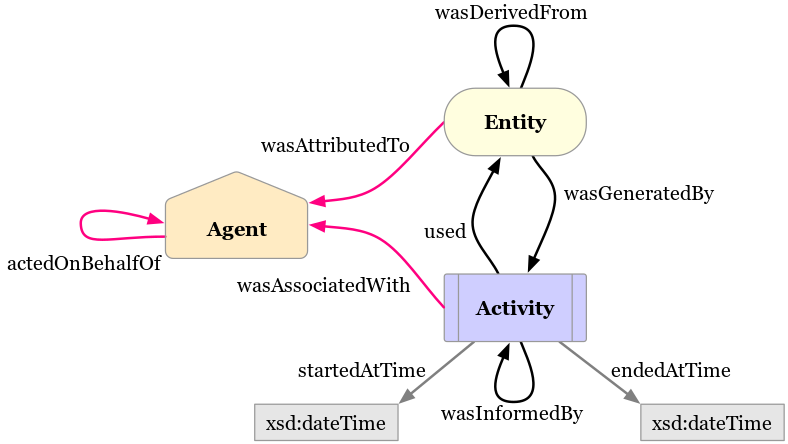
\includegraphics[width=0.8\linewidth]{img/prov-o-model.png}
    \caption{Overview of PROV-O model \cite{lebo_prov-o_2013}}
    \label{fig:prov-o-model}
\end{figure}

PROV-O is a generic and domain independent ontology for representing provenance information.
In order for it to be applied to the domain of GDPR compliance, it needs to incorporate the relevant terminology and enable distinction between different types of activities and entities.
Furthermore, PROV-O as a provenance ontology is intended to represent information about activities that have been executed in the past, and is therefore suitable to represent only the ex-post aspect of GDPR compliance processes.

While PROV-O does provide the concept of \texttt{Plan}\footnote{PROV-O defines a \textit{plan} as a set of actions or steps towards some goal. It clarifies on the lack of concepts relevant to plans as - ``\textit{There exist no prescriptive requirement on the nature of plans, their representation, the actions or steps they consist of, or their intended goals.''}} to represent ex-ante information, it does not provide further concepts or relationships to associate the plan with activities and entities\footnote{PROV-O provides the concept of \texttt{Association} which assigns responsibility to an agent for an activity and indicates that the agent had a role in the activity, which can include a \texttt{Plan} associated using the \texttt{hasPlan} property.}.
In order to adopt PROV-O and use the concept of \texttt{Plan} for representing ex-ante information for GDPR compliance, it needs to be extended with the additional concepts and relationships.

\subsubsection{P-Plan - extending PROV-O Plans as Workflows}
P-Plan \cite{garijo_p-plan_2014} extends the concept of \texttt{Plan} in PROV-O towards representing scientific
workflows which enable creating a template of a `step' and linking it to executions of activities.
A \texttt{p-plan:Plan} is a subclass of \texttt{prov:Plan} and is composed of smaller activities or steps (\texttt{p-plan:Step}) that use and generate (as inputs or outputs) variables (\texttt{p-plan:Variable}).
An overview of the relationship between PROV-O and P-Plan is described in \autoref{fig:p-plan-model}.
P-Plan enables the representation of provenance information associated with both ex-ante and ex-post processes by representing them as scientific workflows. It also enables associating plans with their executions, thereby providing a link between ex-ante and ex-post provenance information.
\begin{figure}[htbp]
    \centering
    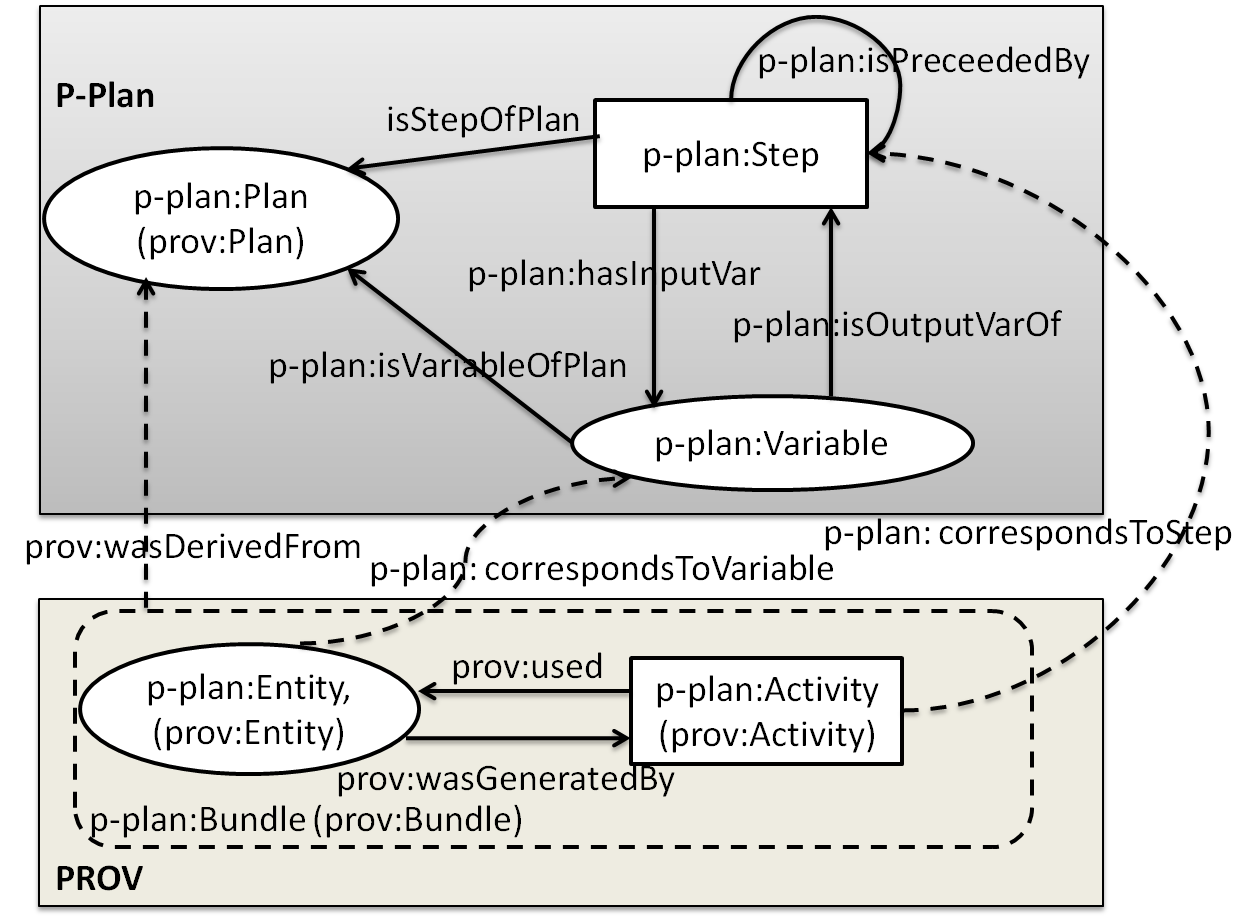
\includegraphics[width=0.75\linewidth]{img/p-plan-model.png}
    \caption{Overview of P-Plan model and its relationship with PROV-O \cite{garijo_p-plan_2014}}
    \label{fig:p-plan-model}
\end{figure}

A \texttt{p-plan:Plan} represents information of `how’ something should happen or a `template’ for executions. A \texttt{p-plan:Activity} is a subclass of \texttt{prov:Activity} and represents the execution of the process described in a \texttt{p-plan:Step}.
A \texttt{p-plan:Entity} is a subclass of \texttt{prov:Entity} that corresponds to a \texttt{p-plan:Variable} in the \texttt{p-plan:Plan}. Therefore, a
\texttt{p-plan:Step} may describe the template including inputs and outputs which can
then be instantiated into multiple instances of \texttt{p-plan:Activity} that can have
distinct inputs to produce different outputs.
As \texttt{p-plan:Plan} extends \texttt{prov:Plan}, which itself extends \texttt{prov:Entity}, it can be
used to treat the \texttt{p-plan:Plan} as an object whose provenance can be tracked using
PROV-O or P-Plan. This makes it possible to express provenance of processes that themselves also describe provenance, thereby creating a history of how plans were formulated and executed over time.

\subsubsection{Extending ontologies for GDPR}
The PROV-O and P-Plan ontologies were extended to represent concepts and relationships of ex-ante and ex-post activities associated with personal data and consent based on requirements of GDPR compliance.
The decision to extend PROV-O and P-Plan with GDPR concepts was made as both ontologies contain generic concepts associated with activities and workflows which can be used for representing information about GDPR compliance, but doing so would be not be intuitive due to the difference in terminology and structuring of information as expected for GDPR compliance.

Extending existing ontologies of PROV-O and P-Plan enables expressing a `template'
or `plan' using \texttt{p-plan:Plan} describing ex-ante activities (as \texttt{p-plan:Step}) that can take place. This template can then be used to denote execution of activities in ex-post phase using \texttt{p-plan:Activity}.
This provides a machine-readable and documented data model of both ex-ante and ex-post activities, whose provenance itself can be expressed (using PROV-O and P-Plan) to record how they were created and how they  change over time.
This is beneficial in documenting the state of a system at a given time as a set of activities that deal with consent and personal data, and
can be helpful in determining changes when the interactions between personal data and an activity change over time.

The extended ontology derived from PROV-O and P-Plan incorporates concepts and relationships associated with GDPR in order to normalise the terminology for representing information associated with GDPR compliance.
The concepts and relationships are derived from the competency questions and linked with their relevant clauses within the GDPR through the use of GDPRtEXT concepts by using \texttt{rdfs:isDefinedBy} and \texttt{rdfs:seeAlso}.
This provides a form of documentation regarding the origin of concepts and their use in the representation of information associated with those clauses of the GDPR.
It also provides a machine-readable link from the ontology to GDPR, which can be used to compare, analyse, and align relevant ontologies.

The extension consists of sub-classing existing concepts in PROV-O and P-Plan to represent specific activities associated with GDPR compliance. 
The use of subclass mechanism preserves the existing concepts and relationships of PROV-O and P-Plan so as to provide compatibility and reuse. This is particularly important in the case of PROV-O as it is the W3C standard for representing provenance information and therefore is more likely to used and expected within the community.
The compatibility also enables packaging the information defined using the ontology as an artefact and defining its provenance as well as planning to provide meta-documentation about how compliance is to be planned and maintained. This is particularly useful to maintain periodic snapshots of organisational processes associated with compliance, and provides the opportunity to automate the querying and validation of information checks within a use-case - as demonstrated in \autoref{chapter:testing}.

\subsection{Ontology Description \& Application}
The resulting ontology is named GDPRov (GDPR Provenance Ontology) and is published online along with its documentation at \url{https://w3id.org/GDPRov/} under the open and permissive CC-by-4.0 license.
The ontology was created, documented, and published using the methodology presented in \autoref{sec:voc:methodology}.
The aim of GDPRov is to provide representations of ex-ante and ex-post activities regarding personal data and consent for GDPR compliance.
It uses the GDPRtEXT ontology to define concepts based on their origin and relevance to clauses within the text of GDPR.

\subsubsection{Overview of GDPRov concepts}
GDPRov extends concepts from PROV-O and P-Plan to represent activities associated with GDPR compliance, with a visual overview provided in \autoref{fig:vocabs:gdprov-overview}.
To that end, it extends the concept of \texttt{p-plan:Plan} in the form of \texttt{Process} to represent ex-ante plans of activities that will take place. The terminology is based on the use of term in commonly used expressions such as `business processes' and `compliance processes'.
Each \texttt{Process} can contain steps (represented by \texttt{p-plan:Step}) to represent activities that interact with data and agents.
To associate steps with a process, the property \texttt{p-plan:isStepOfPlan} is extended as \texttt{isPartOfProcess}.
Another additional property - \texttt{refersToProcess} is also used to enable referring to a process without being a part of it.
Similarly, to associate data (defined in P-Plan as \texttt{p-plan:Variable}) the properties \texttt{p-plan:hasInputVar} and \texttt{p-plan:isOutputVarOf} are extended for activities using inputs and producing outputs respectively.
The ex-post activities in P-Plan are represented by \texttt{p-plan:Activity}.
Data interactions with these activities is represented by \texttt{p-plan:Entity} and the properties \texttt{prov:used} and \texttt{prov:wasGeneratedBy} are used to indicate inputs and outputs respectively.
GDPRov defines steps to indicate automated execution and user interactions regarding collecting data from the user (input) and providing data (output).
To indicate the legal basis associated with a process or a step, the property \texttt{hasLegalBasis} is provided.
\begin{figure}[htbp]
    \centering
    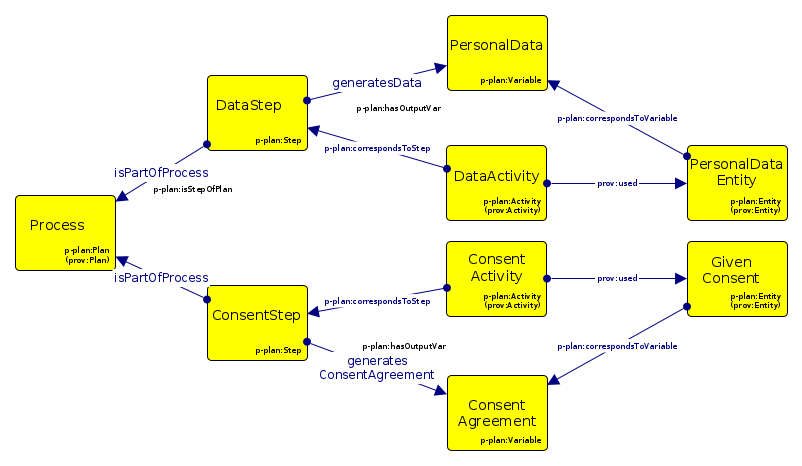
\includegraphics[width=\linewidth]{img/GDProv_relation_prov_pplan.png}
    \caption{GDPRov concepts derived by extending PROV-O and P-Plan}
    \label{fig:vocabs:gdprov-overview}
\end{figure}

\subsubsection{Depicting Data Life-cycle}
Activities associated with the life-cycle of personal data constitute of collecting, processing or using it, storing, sharing, deleting, transferring, transforming, anonymise, and rectifying it. GDPR defines several more categories of actions on data in Article 4-2 in its definition of `processing'.
GDPRov provides broad and abstract processes to represent data access, data archival, data erasure, and data rectification given the need to execute these using several more steps.
GDPRov also provides representations of actions in ex-ante phase as \texttt{DataStep} which extends \texttt{p-plan:Step} and in ex-post phase as \texttt{DataActivity} which extends \texttt{p-plan:Activity}.
These are further extended to distinguish between data collection, data deletion, data sharing, data storage, data archival, data transfer, data transformation, data usage, and rectification of data.
A summary of steps describing a data life-cycle using GDPRov is provided in \autoref{fig:vocabs:gdprov-data-lifecycle}.
\begin{figure}[htbp]
    \centering
    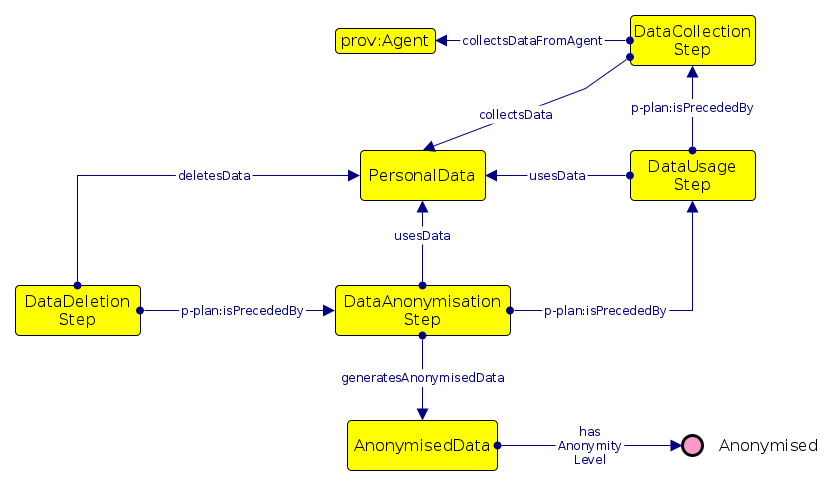
\includegraphics[width=\linewidth]{img/GDPRov_data_lifecycle.png}
    \caption{Example steps depicting data life-cycle using GDPRov}
    \label{fig:vocabs:gdprov-data-lifecycle}
\end{figure}

The anonymisation of data is defined as a sub-class of data transformation to indicate the transformation of data that takes place when anonymising it.
As GDPR obligations are based on the level of anonymity and the capability of de-anonymising it from an organisation's point of view, GDPRov provides the concept of \texttt{anonymisation level} to indicate the state of anonymity the data is in.
GDPRov defines four levels of anonymisation based on existing work in representing anonymous data \cite{hintze_meeting_2017}, which constitute of data that is completely anonymised, completely de-anonymised, pseudo-anonymised, and pseudo-organisational-anonymised where the organisation does not have the data required to de-anonymise it and can thus internally utilise it as if it were completely anonymous data.
The sharing of data consists of interactions with actors or agents, which are represented by \texttt{prov:Agent} and associated with the respective steps and activities using extended properties.

The personal data used within activities is represented by \texttt{PersonalData} which is sub-classed from \texttt{p-plan:Variable} for ex-ante representation and by \texttt{PersonalDataEntity} which is sub-classed from \texttt{prov:Entity} for ex-post representation.
Further categorisation of personal data into anonymised, sensitive, and representing user identifier is provided through sub-classes.

\subsubsection{Depicting Consent Life-cycle}
Activities associated with consent and its life-cycle are represented in ex-ante phase by sub-classing \texttt{p-plan:Step} as \texttt{ConsentStep} and in ex-post phase by sub-classing \texttt{p-plan:Activity} as \texttt{ConsentActivity}.
These are further sub-classed to represent the acquisition, archival, modification, and withdrawal of consent.
Amongst these, withdrawal of consent is defined as sub-class of modification since it modifies the state of consent.
A visual summary of the steps in a consent life-cycle is provided in \autoref{fig:vocabs:gdprov-consent-lifecycle}.
\begin{figure}[htbp]
    \centering
    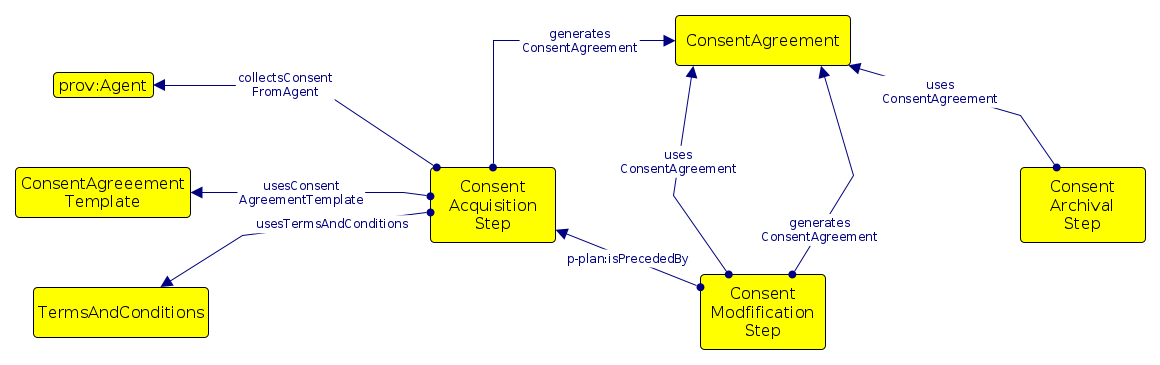
\includegraphics[width=\linewidth]{img/GDPRov_consent_lifecycle.png}
    \caption{Figure describing consent life-cycle defined using GDPRov}
    \label{fig:vocabs:gdprov-consent-lifecycle}
\end{figure}

The artefacts associated with consent and used in activities include the choices or offer of consent provided to the individual and the subsequent consent given by the individual.
To represent these in ex-ante phase, GDPRov provides the concepts of \texttt{ConsentAgreementTemplate} to represent the template offered to collect consent, \texttt{ConsentAgreement} to indicate the given consent, and \texttt{TermsAndConditions} to indicate the policies or terms and conditions.
The corresponding concepts in ex-post phase are \texttt{GivenConsentTemplate}, \texttt{GivenConsent}, and \texttt{TermsAndConditionsEntity}.

\subsubsection{Depicting Compliance-related processes}
In addition to representing activities associated with personal data and consent, GDPRov also provides representations for compliance-related processes.
These include actions such as appointing processor (by a controller), carrying out an impact assessment, marketing and its special case of direct marketing, and monitoring compliance.
Processes are also provided for handling data breaches, which include notifying the controller (by a processor), notifying the data subject, and notifying the data protection authority.
The handling of right provided by the GDPR is represented through sub-classes of \texttt{Process} for data portability, erasure, access personal data, basic info about processing, no automated processing, object to direct marketing, object processing, rectification, restrict processing, transparency, SAR (subject access request).

% \subsubsection{Actors and Agents}
% Controller Representative
% Data Subject
% DPO
% Processor Representative
% Third Party
%     Controller
%         Joint Controller
%     Processor
%         SubProcessor

% \subsubsection{Documentation \& Dissemination}

\subsubsection{Example Use-Case: Querying anonymised sharing of data}
The applicability and usefulness of GDPRov is demonstrated through its use for querying and validation of information for GDPR compliance in \autoref{chapter:testing}.
A simplified example demonstrating such an application through the use of a SPARQL query was published along with the ontology in the peer-reviewed publication \cite{pandit_modelling_2017}, and which is presented in \autoref{code:gdprov:sparql} to demonstrate how GDPRov can assist in the answering of compliance questions for GDPR.
The query uses GDPRov concepts to retrieve data being shared, the specific steps that share it, the anonymisation level of shared data, and the anonymisation steps used to anonymise it. The query is meant to retrieve information relevant in the investigation of data being shared and its anonymity.
\begin{listing}[htbp]
\begin{minted}{sparql}
PREFIX gdprov: <https://w3id.org/GDPRov#>
SELECT ?data ?sharestep ?isAnonymised ?anonymisationStep
WHERE {
    ?data a gdprov:Data .
    ?sharestep a gdprov:DataSharingStep .
    ?sharestep gdprov:sharesData ?data. 
    BIND (
        EXISTS { ?data a gdprov:AnonymisedData . }
        as ?isAnonymised ) .
    OPTIONAL {
        ?anonymisationStep
        gdprov:generatesAnonymisedData ?data .
    }
}
\end{minted}
\caption{SPARQL query representing compliance question \texttt{G5} concerning legal basis for processing}
\label{code:gdprov:sparql}
\end{listing}

\subsubsection{Example Use-Case: Detecting changes in activities for updates to consent}
An example of a use-case is when a data controller updates a plan of processing activities such as when a purpose changes or a new processing operation is added to an existing purpose - and where the legal basis for such processing is consent.
In such cases, the data controller is required to evaluate whether updating an individual's consent is required as per the GDPR based on the changes between the given consent and the new purposes or processing activities. By storing the plans of processing operations using GDPRov, it is possible to compare the old and new versions of a plan, detect changes, and identify whether corresponding updates to consent are needed. 

An exploration of the above change detection was published in the Managing the Evolution and and Preservation of the Data Web workshop co-located with ESWC 2018 \cite{pandit_gdpr-driven_2018} where a model of activities were represented using P-Plan and then compared to identify changes. The use of P-Plan can be substituted with GDPRov when representing GDPR-specific activities.
The publication explored the change when an existing plan is updated to remove the step of sending advertisements. 

The change detection, visualised in \autoref{fig:vocabs:gdprov-change-detection}, is based on identifying the differences between the two plans in terms of steps and variables and whether they have been added, removed, or modified.
In the figure, the change reflects the removal of a step - which by itself does not require any changes to a given consent since no new purposes have been added to an existing given consent.
Using this approach, the detected change can be analysed - manually for complex and legal interpretations while automatically for simpler or simplified graphs - and used to identify whether corresponding changes are necessary based on compliance obligations.
\begin{figure}[htbp]
    \centering
    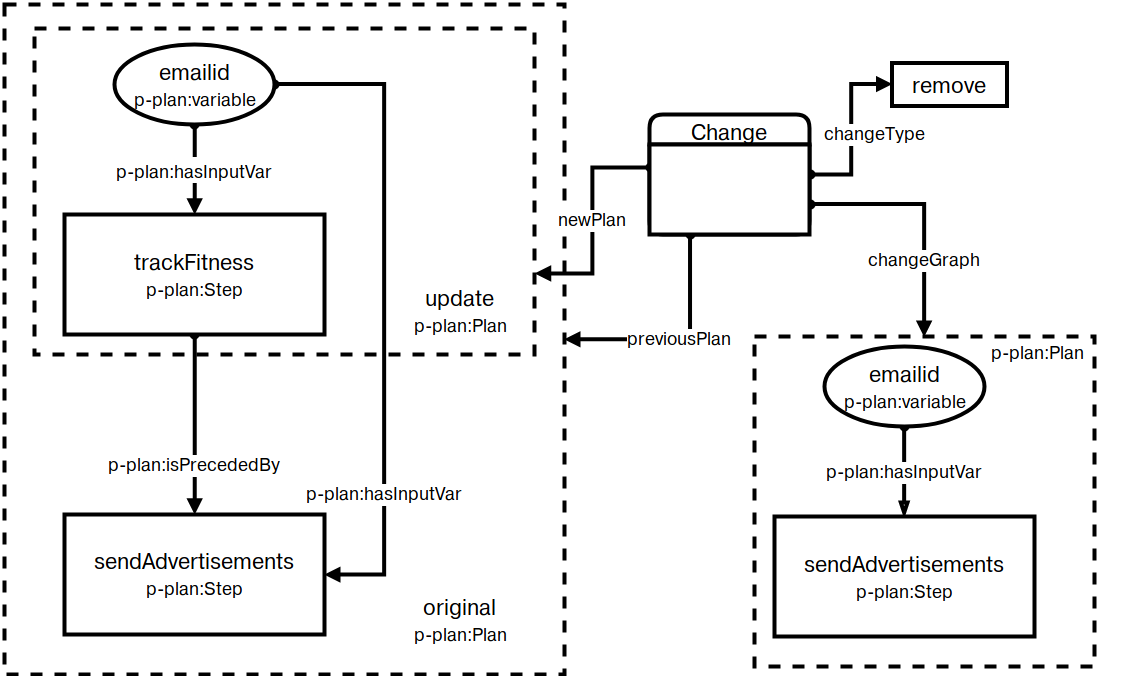
\includegraphics[width=\textwidth]{img/GDPRov-change-detection.png}
    \caption{Modelling changes in workflows using P-Plan \cite{pandit_gdpr-driven_2018}}
    \label{fig:vocabs:gdprov-change-detection}
\end{figure}

\subsection{Evaluation}\label{sec:voc:gdprov:evaluation}
The ontology assessment was based on the methodology outlined in \autoref{sec:voc:methodology} regarding the criterion for evaluation of the quality of ontology and its documentation.
The ontology was used in two applications developed to demonstrate use of SPARQL to query information (see \autoref{sec:testing:sparql}) and SHACL to validate information for GDPR compliance (see \autoref{sec:testing:shacl}). The experience was used to identify suitability of GDPRov in representing the required information, and led to addition of \texttt{ConsentAgreementTemplateBundle} as a concept for convenience in representing `bundled' consent requests and provisions based on consent workflows on a website where a single dialogue is used to collect consent involving multiple distinct purposes and third parties.

GDPRov was published \cite{pandit_modelling_2017} as a peer-reviewed publication in the Workshop on Society, Privacy and the Semantic Web - Policy and Technology (PrivOn) co-located with the 16th International Semantic Web Conference (ISWC). The workshop provided reviews from domain experts in the privacy, legal, and semantic web domains; with ISWC being a top-tier conference in the semantic web domain.

To date, the publication has received 18 citations to date (excluding self-citations) on Google Scholar\footnote{\url{https://scholar.google.com/scholar?cites=2287149512924017207}} of which 2 are deliverables of the CitySPIN research project (see \autoref{sec:sota:gdpr-semweb}).
% Of these, the publications associated with PrOnto \cite{palmirani_pronto_2018,palmirani_pronto_2018-1} incorrectly conclude that ``GDPRov aims to describe the provenance of the consent and data lifecycle in the light of the Linked Open Data principles such as Fairness and Trust'' - since the basis of GDPRov is the scientific workflow model similar to the one used within PrOnto.
% The publication of a PROV-O model representing activities for GDPR compliance by Ujcich et al. \cite{belhajjame_provenance_2018} cites GDPRov as a relevant approach with the comparison to GDPRov specified as - ``Our model allows for more flexible specifications of how data can be used (i.e.,under consent for particular purposes while being legally valid for a period of time). Furthermore, our model focuses on temporal reasoning and online data usage control, whereas it is not clear how amenable GDPRov is to such reasoning or enforcement.'' While the example provided in the publication does provide temporal annotation of activities for GDPR compliance - these are achieved through the use of PROV-O rather than specialised classes using GDPR terminology. Since GDPRov extends PROV-O, it supports such use of inherent PROV-O concepts. In addition, GDPRov provides expression of ex-ante activities and workflows which cannot be expressed using the model proposed by Ujcich et. al.
A publication describing an approach for annotating DFDs (data flow diagrams) with information for analysing compliance \cite{debruyneOntologyRepresentingAnnotating2019}  utilises GDPRov to represent personal data as an entity used in activities. The publication provides an ontology for representation of DFDs to abstract the processing operations as data flows based on the argument of their ease of analysis as compared to workflows.

\subsubsection{Fulfilment of Competency Questions}
An assessment of the extent to which GDPRov satisfies the competency questions by providing concepts and relationships is presented as part of its evaluation.
The competency questions, summarised in \autoref{sec:gdprov:cq}, were used to guide the development of the ontology and therefore used to evaluate if the ontology meets the requirements of representing this information.
\autoref{table:gdprov:cq} lists the concepts and properties relevant to answer the competency question (with \textit{N/S} used to indicate not in scope).
\begin{table}[htbp]
\footnotesize
\centering
\rowcolors{1}{}{gray!10}
\begin{tabularx}{\linewidth}{|l|X|p{5cm}|l|}
\caption{Concepts in GDPRov for answering competency questions} \\ \hline
\label{table:gdprov:cq}
\textbf{CQ} & \textbf{Class} & \textbf{Property} & \textbf{Phase} \\ \hline
\multicolumn{4}{|l|}{\textbf{Actors and Agents involved in activities}}  \\ \hline
\textit{CMQ2} & \textit{Controller}, \textit{ControllerRepresentative}, \textit{DPO} &  &  \\ \hline
\textit{CMQ17} & \textit{Processor}, \textit{ProcessorRepresentative}, \textit{DPO} &  &  \\ \hline
\textit{CMQ35} & \textit{DataSubject} &  &  \\ \hline
\multicolumn{4}{|l|}{\textbf{Details of processing}}  \\ \hline
\textit{CMQ3} & \textit{Process} & \textit{refersToProcess} & \textit{Ex}-\textit{ante} \\ \hline
\textit{CMQ4} & \textit{DataSubject} &  &  \\ \hline
\textit{CMQ5} & \textit{PersonalData}, \textit{SensitiveData} & \textit{usesData} & \textit{Ex}-\textit{ante} \\ \hline
 & \textit{PersonalDataEntity}, \textit{SensitiveDataEntity} &  & \textit{Ex}-\textit{post} \\ \hline
\textit{CMQ6} & \textit{DataSharingStep} & \textit{sharesData}, \textit{sharesDataWith} & \textit{Ex}-\textit{ante} \\ \hline
 & \textit{DataSharingActivity} & \textit{hasSharedDataWith} & \textit{Ex}-\textit{post} \\ \hline
\textit{CMQ7} & \textit{ThirdParty} & \textit{sharesDataWithThirdParty} & \textit{Ex}-\textit{ante} \\ \hline
\textit{CMQ8} & \textit{ThirdParty} & \textit{sharesData}, \textit{sharesDataWith} & \textit{Ex}-\textit{ante} \\ \hline
\textit{CMQ9} & \textit{N}/\textit{S} & \textit{N}/\textit{S} &  \\ \hline
\textit{CMQ10} & \textit{N}/\textit{S} & \textit{N}/\textit{S} &  \\ \hline
\textit{CMQ11} & \textit{DataStorageStep} & \textit{usesData}, \textit{generatesData} & \textit{Ex}-\textit{ante} \\ \hline
 & \textit{DataStorageActivity} &  & \textit{Ex}-\textit{post} \\ \hline
\textit{CMQ12} & \textit{N}/\textit{S} & \textit{N}/\textit{S} &  \\ \hline
\textit{CMQ13} & \textit{N}/\textit{S} & \textit{N}/\textit{S} &  \\ \hline
\textit{CMQ26} &  & \textit{hasLegalBasis} &  \\ \hline
\multicolumn{4}{|l|}{\textbf{Lifecycle of data}} \\ \hline
\textit{CMQ28} & \textit{DataCollectionStep} & \textit{collectsData} & \textit{Ex}-\textit{ante} \\ \hline
 & \textit{DataCollectionActivity} &  & \textit{Ex}-\textit{post} \\ \hline
\textit{CMQ29} & \textit{DataCollectionStep} & \textit{collectsDataFromAgent} & \textit{Ex}-\textit{ante} \\ \hline
 & \textit{DataCollectionActivity} & \textit{collectedDataFromAgent} & \textit{Ex}-\textit{post} \\ \hline
\multicolumn{4}{|l|}{\textbf{Anonymisation}} \\ \hline
\textit{CMQ31} & \textit{DataAnonymisationStep}, \textit{AnonymisedData} &  & \textit{Ex}-\textit{ante} \\ \hline
 & \textit{DataAnonymisationActivity}, \textit{AnonymisedDataEntity} &  & \textit{Ex}-\textit{post} \\ \hline
\textit{CMQ32} & \textit{PersonalData}, \textit{SensitiveData} & \textit{hasAnonymityLevel} & \textit{Ex}-\textit{ante} \\ \hline
\multicolumn{4}{|l|}{\textbf{Activities associated with Consent}} \\ \hline
\textit{CMQ48} & \textit{ConsentStep}, \textit{ConsentAcquisitionStep}, \textit{ConsentModificationStep}, \textit{ConsentArchivalStep}, \textit{ConsentAgreement}, \textit{ConsentAgreementTemplate} & \textit{usesConsentAgreement}, \textit{generatesConsentAgreement} & \textit{Ex}-\textit{ante} \\ \hline
 & \textit{ConsentActivity}, \textit{AcquireConsentActivity}, \textit{ArchiveConsentActivity}, \textit{ModifyConsentActivity}, \textit{GivenConsent}, \textit{GivenConsentTemplate} & \textit{collectedConsentFromAgent} & \textit{Ex}-\textit{post} \\ \hline
\textit{CMQ49} & \textit{ConsentAgreementTemplate} &  & \textit{Ex}-\textit{ante} \\ \hline
 & \textit{GivenConsentTemplate} &  & \textit{Ex}-\textit{post} \\ \hline
\end{tabularx}
\end{table}

% Some questions which were not considered in scope regarding expression of activities are marked with \textit{N/S}. 
Questions not in scope (marked as \textit{N/S} either require clarity from authoritative sources regarding interpretation of information to provide a concrete design pattern or have multiple possible representations of which it cannot be determined which is more useful from a legal compliance point of view. Examples include location of recipients - which can be expressed either through an property/annotation associated with a data sharing activity or attached with a particular third party; and specifying time limits or duration or conditional events associated with data storage and deletion periods. These have been identified as future work regarding further development of the ontology based on differing interpretations of representation, complexity of specifying values such as ``EU membership'' and  ``as long as required'', and the pending expert opinion of legal authorities on these issues through courts or executive decisions.

The presented evaluation demonstrates GDPRov satisfies the requirements of answering competency questions regarding representation of activities and identifies those that are needed to be resolved as future work based on availability of legal opinion and decisions. GDPRov thus fulfils the research objective $RO3(b)$ by providing representations of activities associated with personal data and consent in ex-ante and ex-post phases.

\subsubsection{Comparison with SotA}
The representation of process flows and activities associated with GDPR compliance in existing approaches was presented and analysed as part of the state of the art in \autoref{sota:analysis:process-flows}.
The attributes for this analysis involved the features or concepts that could be represented using the specified approach and the basis for the representation in existing vocabularies and standards.
The analysis demonstrated the existence of a variety of approaches that utilised the existing standards of PROV-O and BPMN to model GDPR-specific information regarding process flows and activities in both ex-ante and ex-post phase. It was also found that approaches modelling both ex-post and ex-ante phases exist and utilise PROV-O as their basis for representation of information.

A comparison of GDPRov with the SotA is provided in \autoref{table:gdprov:sota} using the same attributes used for analysis.
The table lists the features supported by each approach through the notation of a check mark (\cmark).
The column headings corresponding with expression of information supported by an approach, and use the following abbreviations - (Repr): method used for representation of process flow; (EA): whether it permits Ex-ante modelling; (EP): whether it permits Ex-post modelling; (Pu): whether Purpose can be specified; (Pr): whether Processing can be specified; (DS): if Data Sharing can be modelled; (Rp): if Recipients are associated with data sharing; (St): whether Data Storage occurs; (Rg): if provision of Rights can be modelled; and (LB): if Legal Basis can be associated with a process flow.
% Table GDPRov vs SotA
\begin{table}[htbp]
\footnotesize
\centering
\rowcolors{1}{}{gray!10}
\begin{tabularx}{\textwidth}{|l|l|X|X|X|X|X|X|X|X|X|}

\caption{Comparison of GDPRov with SotA}\label{table:gdprov:sota} \\ \hline
\textbf{Work} & \textbf{Repr} & \textbf{EA} & \textbf{EP} & \textbf{Pu} & \textbf{Pr} & \textbf{DS} & \textbf{Rp} & \textbf{St} & \textbf{Rg} & \textbf{LB} \\ \hline
\rowcolor[gray]{0.8}
\textbf{GDPRov} & PROV-O,P-Plan & \cmark & \cmark & \cmark & \cmark & \cmark & \cmark & \cmark & \cmark & \cmark  \\ \hline
SPECIAL & PROV-O & \cmark & \cmark & \cmark & \cmark & \cmark & \cmark & \cmark &  &  \\ \hline
SPL+CitySPIN & PROV-O & \cmark & \cmark & \cmark & \cmark & \cmark & \cmark & \cmark &  &  \\ \hline
MIREL & PWO & \cmark &  & \cmark & \cmark &  &  & \cmark & \cmark &  \\ \hline
MRL+DAPRECO & PWO & \cmark &  & \cmark & \cmark &  &  & \cmark & \cmark &  \\ \hline
BPR4GDPR &  & \cmark & \cmark & \cmark & \cmark & \cmark & \cmark &  &  &  \\ \hline
Ujcich et al. & PROV-O &  & \cmark & \cmark & \cmark & \cmark & \cmark & \cmark & \cmark & \cmark \\ \hline
Lodge et al &  & \cmark &  & \cmark &  &  &  &  &  &  \\ \hline
Tom et al & BPMN & \cmark &  &  & \cmark & \cmark & \cmark & \cmark & \cmark &  \\ \hline
LUCE &  & \cmark & \cmark &  &  & \cmark & \cmark &  &  &  \\ \hline
Sion et al &  & \cmark &  & \cmark & \cmark & \cmark & \cmark & \cmark &  & \cmark \\ \hline
privacyTracker &  & \cmark & \cmark &  &  & \cmark & \cmark &  &  &  \\ \hline
Basin et al &  & \cmark &  & \cmark &  &  &  &  &  &  \\ \hline
RestAssured &  &  &  & \cmark & \cmark & \cmark & \cmark & \cmark &  &  \\ \hline
\end{tabularx}
\end{table}

The table demonstrates that GDPRov supports all of the features, and is the only one currently providing all of them. However, this analysis only takes into consideration the abstract existence or provision of features and does not take into consideration the context of the approach or its granularity. For example, while an approach may provide representation of data storage concepts, there are additional features such as storage duration, condition, form or medium, security, and policy which are also relevant to the evaluation of GDPR compliance.
These are highly dependant on individual use-cases and domains, and contain existing work which can be used to represent them such as the Time ontology \cite{cox_time_2017} for temporal annotations and the ODRL ontology \cite{iannella_odrl_2018} for policies.
Since the scope of GDPRov is limited to the expression of information regarding activities in ex-ante and ex-post phases, the representation of such granular attributes is not within the scope and is therefore not considered in its evaluation or comparison with the SotA.

Regarding the expression of information as being in either ex-ante or ex-post phase - GDPRov is the only approach to do so using the existing ontologies of PROV-O and P-Plan based on the scientific workflow model which is useful in the investigation of executions based on a plan and the association of information between ex-ante and ex-post phases. The use of PWO \cite{gangemi_publishing_2017} in the MIREL project also follows a similar rationale though it does not provide the same extent of concepts and representations as GDPRov.
In addition, the utilisation of PROV-O as its base ontology enables information represented using GDPRov to be captured and recorded as provenance information using PROV-O or GDPRov itself. This provides capabilities for documentation the evolution of a system as well as representation the state of compliance at a given moment in time.
This feature is shared by all approaches that utilise a provenance based ontology at their core, and especially the ones that utilise PROV-O as it is a well-recognised and adopted standard.
The combination of PROV-O and P-Plan enables a flexible representation of activities by specifying their constituent steps and involved artefacts at an arbitrary level of granularity while providing annotations and classes to link these with the GDPR. In this, GDPRov is unique and novel within the SotA.

Based on this, GDPRov's novelty within the SotA is based on it being one of the few approaches using PROV-O to represent activities for GDPR compliance in both ex-ante and ex-post phases. GDPRov is also novel in its provision of concepts associated with GDPR and the arbitrary granularity afforded by the use of PROV-O and P-Plan to link information in ex-ante and ex-post phases.
Furthermore, GDPRov is one of the few approaches to be available under an open and permissive license (CC-by-4.0) thereby enabling its use, adoption, and further evolution.

\subsubsection{Application to external use-case from SPECIAL project}\label{sec:gdprov:use-case:SPECIAL}
% description of the use-case
The SPECIAL project uses a scenario\footnote{NOTE: the scenario explicitly mentions use of an immutable distributed ledger developed by the SPECIAL project to provide transparency and log accountability regarding metadata. This is omitted from the adapted use-case used to evaluate GDPRov.} to motivate their work and demonstrate the use of developed technologies in their deliverables (D1.7 \cite{bonatti_d1.7_2018}) and peer-reviewed publications (\cite{kirrane_scalable_2018}).
In this section, the scenario is adapted as an external use-case to evaluate GDPRov's suitability to express the required concepts.

The use-case is summarised as follows with GDPR concepts added in parenthesis for relevance: Sue (Data Subject) buys a wearable appliance for fitness tracking from BeFit (Data Controller), and is presented with an informed consent request that describes collection of biomedical parameters such as heart rate (Personal Data), and how they will be processed, stored in BeFit's cloud and transmitted for the purposes of: giving Sue feedback on her activity, such as calories consumption; and creating an activity profile that will be shared with other companies for targeted ads related to fitness - an optional purpose which Sue opts-in. After two years, Sue starts receiving annoying SMS messages from a local gym that advertise its activities. Sue discovers the following facts: (i) the gym has an activity profile referring to Sue, that, due to the appliance’s malfunctioning, reports that she is not doing any physical exercise; (ii) the gym received the profile from BeFit, associated with a policy that allows the gym to send targeted ads to Sue based on the profile; (iii) BeFit built the profile by mining the data collected by the appliance; and (iv) all these operations are permitted by the consent agreement previously signed by Sue and BeFit. Using this information BeFit and the gym prove that they used Sue’s data according to the given consent. Sue now asks both BeFit and the gym to delete all of her data. 

The use-case is accompanied with information on its interpretation in terms of GDPR terminology \cite{bonatti_d1.7_2018} and its representation using the SPECIAL vocabularies \cite{kirrane_scalable_2018}. To represent the use-case using GDPRov, the concepts used by SPECIAL are mapped or aligned to their closest relative concepts within GDPRov (see \autoref{table:gdprov:use-case:SPECIAL}) with its RDF/Turtle representation provided in \autoref{code:gdprov:use-case:special}. The SPARQL queries used to retrieve information depicted by statements (i) to (iv) in the scenario are provided in \autoref{code:gdprov:use-case:special-sparql}. The RDF representation and SPARQL query utilised a simplified representation of the scenario to present only the facts essential to the answering of questions. 
\begin{center}
\footnotesize
\begin{tabularx}{\textwidth}{|p{0.35\linewidth}|X|X|}
\caption{GDPRov concepts to represent external use-case from SPECIAL} \label{table:gdprov:use-case:SPECIAL} \\
\toprule
\textbf{Statement} & \textbf{GDPRov concept} & \textbf{SPECIAL concept} \\
\midrule
\endhead
Sue & \texttt{DataSubject} & \texttt{DataSubject} \\ \hline
BeFit & \texttt{DataController} & \texttt{Controller} \\ \hline
Biomedical parameters, heart rate, calories consumption, activity profile & \texttt{PersonalData} & \texttt{Data} \\ \hline
Collect data & \texttt{DataCollectionActivity} & \texttt{Collect} \\ \hline
Provide feedback on activity & \texttt{Purpose} & \texttt{Purpose} \\ \hline
Give consent (opt-in) & \texttt{AcquireConsentActivity} & \texttt{ConsentAssertion} \\ \hline
Targeted ads related to fitness & \texttt{Purpose} & \texttt{Purpose} \\ \hline
Share data & \texttt{DataSharingActivity} & \texttt{Recipient} \\ \hline
Gym & \texttt{ThirdParty} & \texttt{Recipient} \\ \hline
Consent agreement & \texttt{GivenConsent} & \texttt{LogEntryContent} \\ \hline
Delete data & \texttt{DataDeletionActivity} & N/A \\ \hline
Withdraw consent & \texttt{WithdrawConsentActivity} & \texttt{ConsentRevocation} \\
\bottomrule
\end{tabularx}
\end{center}
\begin{listing}[htbp]
\begin{minted}{turtle}
# Entities
:Sue a gdprov:DataSubject .
:BeFit a gdprov:DataController .
:Gym a gdprov:ThirdParty .
# Personal Data
:Biomedical_Parameters a gdprov:PersonalData .
:Activity_Profile a gdprov:PersonalData .

# Register with BeFit, given consent, and generate activity profile
:Registration a gdprov:Process .
:Sue_consent a gdprov:GivenConsent, gdprtext:LawfulBasisForProcessing .
:Collect_consent a gdprov:AcquireConsentActivity ;
    gdprov:isPartOfProcess :Registration .
    gdprov:collectedConsentFromAgent :Sue ;
    gdprov:generatedConsent :Sue_consent .
:Collect_data a gdprov:DataCollectionActivity ;
    gdprov:isPartOfProcess :Registration ;
    prov-o:wasInformedBy :Collect_consent ;
    gdprov:collectedDataFromAgent :Sue ;  # from Sue's device
    gdprov:generatedData :Activity_Profile .

# Share activity profile with Gym
:Targeted_ads_related_to_fitness a gdprov:Process ;
    gdprov:hasLegalBasis :Sue_consent .
:Share_data a gdprov:DataSharingActivity ;
    :sharedData :Activity_Profile ;
    :hasSharedDataWith :Gym .
# Gym receives Sue's activity profile from BeFit
:Collect_data_from_BeFit a :DataCollectionActivity ;
    gdprov:collectedDataFromAgent :BeFit ;
    gdprov:involvesAgent :Sue ;
    gdprov:refersToProcess :Targeted_ads_related_to_fitness ;
    gdprov:generatedData :Activity_Profile . # Gym copy of data

# Sue withdraws consent
:Withdraw_consent a gdprov:WithdrawConsentActivity ;
    prov:invalidated :Sue_consent .
# BeFit and Gym deleted the activity profile
:Delete_data a gdprov:DataDeletionActivity ;
    prov:invalidated :Activity_Profile ;
    prov:wasInformedBy :Withdraw_consent .
\end{minted}
\caption{GDPRov representation of external use-case from SPECIAL}
\label{code:gdprov:use-case:special}
\end{listing}
\begin{listing}[htbp]
\begin{minted}{sparql}
# Query (i)
# retrieves :Activity_Profile as personal data shared with Gym
# queried over Gym's records
SELECT ?personal_data 
WHERE {
    ?personal_data a gdprov:PersonalData .
    ?activity gdprov:generatedData .
    ?activity (gdprov:collectedDataFromAgent|gdprov:involvesAgent) :Sue .
}

# Query (ii)
# retrieves :BeFit as data source
# retrieves :Targeted_ads_related_to_fitness as purpose
# queried over Gym's records
SELECT ?party, ?purpose 
WHERE {
    ?activity gdprov:generatedData :Activity_Profile .
    ?activity gdprov:collectedDataFrom ?party .
    ?activity gdprov:refersToProcess ?purpose .
}

# Query (iii)
# retrieves :Sue as data source (as Sue's device)
# queried over BeFit's records
SELECT ?data_source 
WHERE {
    ?activity_profile gdprov:generatedData :Activity_Profile .
    ?activity_profile gdprov:collectedDataFromAgent ?data_source .   
}

# Query (iv)
# retrieves :Sue_consent as the legal basis for data collection and mining
# queried over BeFit's records
SELECT ?legal_basis 
WHERE {
    {
        ?activity gdprov:generatedData :Activity_Profile .
    } UNION {
        ?activity gdprov:sharedData :Activity_Profile .
        ?activity gdprov:hasSharedDataWith :Gym .
    }
    ?activity (
            gdprov:hasLegalBasis|
            (gdprov:isPartOfProcess/gdprov:hasLegalBasis))
        ?legal_basis .
}


\end{minted}
\caption{SPARQL queries using GDPRov for external use-case from SPECIAL}
\label{code:gdprov:use-case:special-sparql}
\end{listing}

Through the representation of the concepts within the scenario and the use of SPARQL, GDPRov is shown to support the representation and answering of questions within the scenario. While the scenario relies on the use of SPECIAL's policy-based vocabulary and the immutable distributed ledger to store and retrieve information regarding given consent and the processing activities carried out by BeFit and the Gym, these have not been replicated the above representation as storage mechanisms are not within scope for this work.

One important conclusion from the above exercise is the representation of given consent, where SPECIAL vocabularies represent the given consent as a policy using OWL2 \cite{kirrane_scalable_2018}.
In comparison, GDPRov does not represent information provided in the consent request and given consent, but instead records it as an activity and associates the generated consent as an artefact representing a legal basis with the purposes (specified using \texttt{gdprov:Process}) that rely on it. 
This is the consequence of GDPRov focusing on the representation of activities which does not concern the representation of consent.
A consent-centric representation of this same scenario is presented in \autoref{sec:gconsent:use-case:SPECIAL} which uses GConsent to represent the scenario as interactions between consent states.

% \subsubsection{Application to external use-case from Ujcich et al.}
% Ujcich et al. present a similar (to the above) scenario in their demonstration of a provenance vocabulary based on the GDPR \cite{belhajjame_provenance_2018}. 
% The scenario concerns Alice, a customer, who registers with a retailer and provides name, address, and credit card number; gives consent to store these and use for purchases made, and also consents to use of name and address to receive marketing. 
% At some period of time, the retailer employs a third-party for marketing and provides it with Alice’s name and address based on the given consent.
% After some more period of time, Alice no longer wishes to receive marketing and withdraws her consent.
% The investigation of compliance presented in the publication utilises two questions related to the scenario, which are: (i) Was Alice’s personal data used for marketing purposes after Alice withdrew her consent?; and (ii) Was Alice’s personal data used for marketing purposes after Alice withdrew her consent?

% Ujcich et al. represent the scenario as a series of activities using PROV-O

% % breakdown into requirements
% % select concepts from GDPRov to represent requirements - ex-ante and ex-post
% % representation Turtle code
% % analysis - what is possible and what isn't
% % comment on deficiencies or advantages of GDPRov

% \subsubsection{Application to External Use-case: Ujcich et al.}
% % description of the use-case
% % breakdown into requirements
% % select concepts from GDPRov to represent requirements - ex-ante and ex-post
% % representation Turtle code
% % analysis - what is possible and what isn't
% % comment on deficiencies or advantages of GDPRov

\subsection*{Summary}
GDPRov is part of the second major contribution of this thesis. It provides an ontological representation of ex-ante and ex-post activities associated with personal data and consent for GDPR compliance.
It thus fulfils the research objective $RO3(b)$ as outlined in \autoref{sec:intro:RQ}. 
The use of GDPRov makes it possible to indicate the plans associated with how personal data and consent is collected, used, stored, shared, and erased.
It also enables the representation of logs for activities that act over personal data and consent.

At the time of this undertaking (in 2016-2017), no other vocabulary was found that represented information about activities associated with GDPR compliance.
The work presented as state of the art in \autoref{chapter:sota} and demonstrating existence of approaches for representing information about GDPR processes were published after the publication of GDPRov. Of these approaches, some also utilise PROV-O to represent provenance of activities as seen through the analysis presented in \autoref{sota:analysis:process-flows}. The differentiating factor of GDPRov is the use of PROV-O and P-Plan as distinct ontologies representing ex-ante and ex-post phases of activities based on the scientific workflow model - which is novel within the state of the art. Another differentiating factor is the use of GDPRtEXT to define concepts and relationships within GDPRov, thereby linking the use of ontology with the legal concepts it was derived from.

Approaches within the state of the art, for example SPECIAL (\autoref{sec:sota:SPECIAL}), demonstrate the applicability of provenance vocabularies in maintaining, querying, and assessing provenance logs represented using PROV-O for GDPR compliance.
While SPECIAL also provides ex-ante compliance assessment by using the same data model and logging it as a request instead of execution \cite{dullaert_d3.4_2019}, GDPRov further expands on the use of provenance to include the representation of plans or templates to indicate the association between activities in ex-ante and ex-post phases of compliance.
% GConsent
\section{GConsent - Ontology of Consent Information for GDPR Compliance}\label{sec:voc:GConsent}
GConsent is a semantic web ontology for representing contextual information about consent based on requirements of GDPR compliance. 
GConsent aims to model the context, state, and provenance of consent as an entity.
Its scope is limited to consent as defined in the GDPR and is intended towards assisting in the modelling of information associated with compliance.
It uses GDPRtEXT to denote the origin and relevance of its concepts within the text of the GDPR.

GConsent is the outcome of applying the methodology presented in \autoref{sec:voc:methodology} to identify and represent information about consent and its life-cycle as required to determine compliance.
For this, the information presented in \autoref{chapter:background} was used to identify the validity of consent defined by GDPR with the requirements and compliance questions presented in \autoref{chapter:information} used as competency questions.
GConsent is published online\footnote{\url{https://w3id.org/GConsent}} with its documentation under the open and permissive license of CC-by-4.0 and its code repository\footnote{\url{https://github.com/coolharsh55/GConsent/}}.

The design of GConsent was influenced by a real-world use-case for managing the consent information based on GDPR compliance requirements, as mentioned earlier in \autoref{sec:info:compliance-questions-methodology}.
In particular, the design of the ontology underwent several iterations based on whether the ontology should model an association or dependency between purposes and processing operations associated with consent. The final iteration, presented here, provides a separation between purpose and processing operations - which is similar to the other representations of consent within the SotA.

\subsection{Distinction with existing work in state of the art}
Information about consent needs to be maintained and shared by multiple parties which includes the data subject who gives consent, controller who uses it as a legal basis, processor who might be collecting from, and authorities who would evaluate its validity. This requires the information about consent across its life-cycle to be maintained in an representation that is interoperable as outlined in the model in \autoref{sec:info:model}.

From the existing work analysed in state of the art in \autoref{chapter:sota}, the focus of approaches for consent is mostly on the concept of `given' consent i.e. consent provided by the data subject and used as a legal basis by the controller. There is a lack of work regarding representing other `states' of consent within its life-cycle as an entity or representation of agreement which are relevant to its use as a legal basis in the determination of processing of personal data and its compliance under GDPR.
Examples of such states are `not given', `refused', `withdrawn' which cannot be modelled in the same manner as `given consent' as they do not reflect the same information as given consent but are still relevant when associated with a particular instance of processing the data subject's personal data. The state of a consent reflects its status for use as legal basis and is also relevant in the management of information from an organisation's perspective.

Apart from the notion of states, the existing approaches also lack modelling representations for events such as delegation, and associations with third parties regarding consent which have an effect on its validity regarding compliance.
GConsent aims to fill this gap, and therefore to provide novelty and contribution by representing a more cohesive and complete representation of information associated with consent under the GDPR.

\subsection{Relationship with GDPRov}
GConsent builds upon and is complimentary to the representation of consent in GDPRov.
The definition of consent as an entity involved in activities is sufficient to express its life-cycle and provenance by using GDPRov. This includes the ex-ante representation of information provided to collect consent and its subsequent agreement by the individual to produce given consent, which is then used within activities as a legal basis, and may be modified, withdrawn, or revoked - signalling its effective end of life-cycle.
While GDPRov is sufficient to represent these states of consent as an entity along with information about activities acting on it, the primary focus of GDPRov is about expressing the information from the point of view of recording its use within activities.
Managing consent as a legal basis involves consideration of information such as purpose of processing, recipients, and contextual information such as medium of provision and collection, and situations such as delegation.

GConsent aims to provide a consent-centric representation of these information categories by providing concepts relevant to the resolution of valid consent as defined by requirements of GDPR compliance. In this, the use of provenance concepts show an overlap with GDPRov.
This is resolved through the differing scopes of the two ontologies, where concepts defined within GDPRov can also be defined using corresponding concepts in GConsent and vice-versa. An example of such cohesive usage is demonstrated through the application of developed ontologies for querying and validation of information in \autoref{chapter:testing}.
By having separation between GDPRov and GConsent, the ontologies are modular and therefore provide an adopter the ability to choose only one of them without involving the other.

\subsection{Requirements Gathering and Establishment of Competency Questions}
The scope of consent as represented within GConsent is limited to the definition of consent as provided by Article 4-11\footnote{In this definition, consent is expressed as the indication of a data subject's wishes regarding processing of their personal data. However, this is a legal definition rather than a semantic one as it essentially defines the set of conditions required to be satisfied by some consent before it is considered valid under GDPR. Additionally, `consent' as a social concept has a pre-defined meaning based on its use in the social context. Therefore, referring to consent in the context of GDPR does not only mean given consent but includes all information and states associated with consent which can then be evaluated to assess whether it fits the definition of consent as a legal basis. Technical approaches can use `consent' to indicate the given consent or the set of all consent states within its life-cycle.} of GDPR. 
Other special cases of consent not included within the scope consist of consent defined by Article 9 regarding use of special categories of personal data, Recital 33 regarding use of personal data for scientific research, and Article 8 along with Recital 38 regarding use of children’s personal data.
These were not included within the scope due to their additional requirements and complexity regarding interpretation and representation using semantic web. Additionally, the current lack of real-world use-cases reflecting how these types of consent would function and the legal guidance on their compliance requirements is noticeably absent in the context of GDPR.

GConsent is primarily based on the notion of consent as a legal basis under Article 6 of the GDPR. The conditions defined in Article 7, Recital 42, and Recital 43 provide the requirements for consent to be considered or determined valid as per the requirements of GDPR.
The Data Controller bears the burden of demonstrating proof and satisfaction of requirements for consent to be considered valid as per Recital 42. This requires demonstrable proof that the data subject provided the consent and that it was valid as per the obligations specified in the GDPR.

For consent to be informed it is necessary to provide information to the data subject which includes the specific purposes of processing the personal data.
GDPR also provides data subjects with the right to modify or withdraw consent as defined in Article 7-3.
When consent is withdrawn the processing carried out done prior to the withdrawal is considered valid under the given consent which was in effect as the legal basis during that period of time.

Through this, a rudimentary summary of information or attributes associated with `consent' as defined by GDPR is expressed as:
\begin{itemize}
    \item Data Subject the consent is about
    \item Personal Data associated with consent
    \item Processing operations or categories the consent is about
    \item Purposes the consent is about
    \item Entity/Agent/Actor the consent is provided to
    \item Specific operations, including data storage and data sharing
    \item Recipients of data or categories of recipients if any
\end{itemize}
These attributes are sufficient to provide a simplified representation of consent, and are used in existing approaches within the state of the art - such as the model of consent in SPECIAL vocabularies \cite{bonatti_special_2018}. However, these attributes are not sufficient by themselves to determine the validity of consent as they lack information about the context the consent was given in as well as changes to its state.

Therefore, further attributes associated with consent are identified and expressed as:
\begin{itemize}
    \item Entity/Agent/Actor that provided the consent - relevant in the case of delegation
    \item Entity/Agent/Actor that revoked, withdrew, or invalidated the consent - relevant in the case of delegation, and authoritative actions such as by regulators or courts
    \item Status of consent at a given period in time
    \item Contextual information regarding request and giving of consent such as - location, medium, timestamp, expiry
    \item Contextual information regarding revocation, withdrawal, and invalidation of consent such as - location, medium, timestamp, expiry
\end{itemize}
In addition to these, the provenance of how consent was requested and obtained is also important.
Specifically, the information about the specific process and artefacts used in the provision of request for consent - which must satisfy the GDPR qualitative requirements such as the request being clearly stated and being unambiguous.

To derive the required concepts, competency questions were identified from the compliance questions presented in \autoref{sec:info:compliance-questions} pertaining to given consent (\texttt{CMQ35-CMQ69}) and change in consent state (\texttt{CMQ70-CMQ87}).
These refer to information regarding consent (e.g. \texttt{CMQ35-CMQ40}), the consent was created/given/changed/invalidated (e.g. \texttt{CMQ41-CMQ52}), the context of how consent was created/given/invalidated (e.g. \texttt{CMQ53-CMQ56}), and third parties associated with the consent (e.g. \texttt{CMQ57-CMQ58}).

\subsection{Ontology Description \& Application}
\subsubsection{Core Concepts}
The core concepts and relationships in GConsent describe the common and primary attributes associated with consent.
In this case, `consent' by itself does not refer to only the state of `given consent' but also stands as a representation of consent whose state is unknown or is refused, withdrawn, or invalidated by the Data Subject, Controller, or an authority such as the court. This definition of consent is based on managing consent as a data entity rather than as a semantic concept. 
The core concepts are associated with consent in all its states and refer to the information necessary to express what the consent is about. This comprises of the 5 attributes visualised in \autoref{fig:vocabs:gconsent-core} - Data Subject, Personal Data, Purpose, Processing, and Status.
\begin{figure}[htbp]
    \centering
    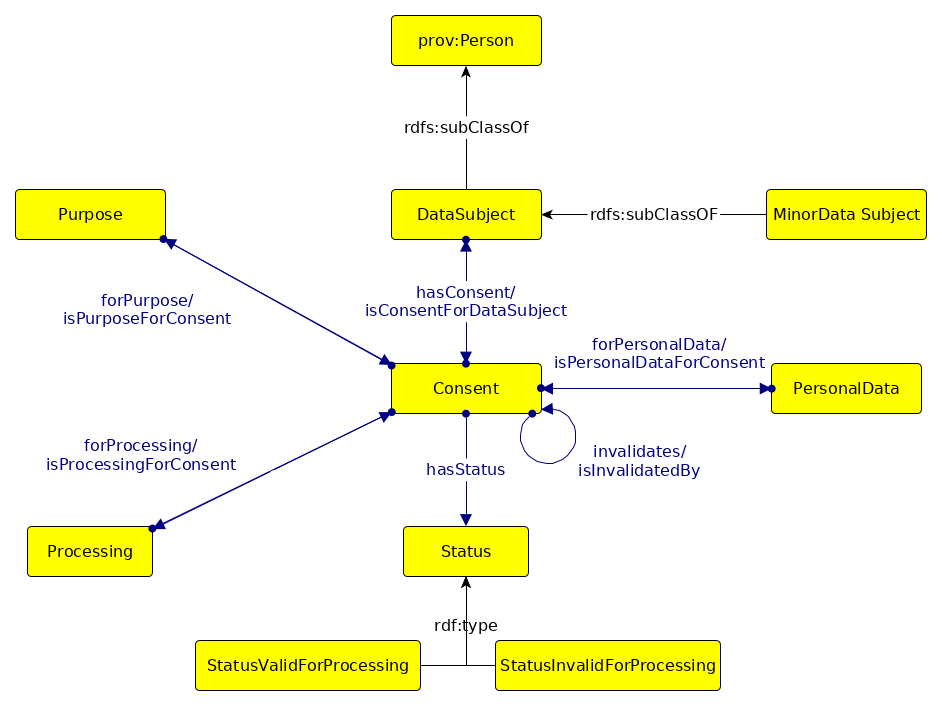
\includegraphics[width=0.8\linewidth]{img/gconsent_core.png}
    \caption{Core concepts in GConsent \cite{pandit_gconsent_2019}}
    \label{fig:vocabs:gconsent-core}
\end{figure}

The \texttt{DataSubject} is the person the consent is associated with as an agreement of their choices. This person may or may not be the same entity that gave the consent - as in the case of parent or guardian giving consent for a child or the act of delegation. The \texttt{DataSubject} class is defined as a subclass of \texttt{prov:Person}, and has the subclass \texttt{MinorDataSubject} to denote a data subject that is legally a minor or a child.
Each instance of \texttt{Consent} is associated with one and only one \texttt{DataSubject}, and any further changes or modifications to the state of consent will continue to be associated with the same \texttt{DataSubject}.
The \texttt{PersonalData} is the set of personal data associated with the consent. Where multiple personal data are associated with a single instance of consent, it is interpreted to mean the union of these sets of personal data. Similarly, \texttt{Purpose} and \texttt{Processing} are also to be interpreted as union rather than intersection.
The `status' or `state' of consent indicates the suitability of using that specific instance of consent as a legal basis for the processing of personal data defined by the consent attributes.

\texttt{Purpose} and \texttt{Processing} are concepts that have semantic meaning based upon their use within the GDPR.
`Processing' is defined by Article 4-2, while `Purpose' has no specific definition provided but can be summarised as the intent or aim of why the set of personal data is needed or to be used for. In practice, purpose is generally defined at a higher abstract level, and often encompasses several types or categories of data. An example of this is a privacy policy specifying `account information' and `location of service use' - which are data categories, that are `collected' and `used' - which are processing operations on the personal data, `to ensure security of the account' - which is the purpose the personal data will be processed for. The relation between a purpose and its associated processing operations is quite opaque when considered as a purpose involving one or more processing operations. Based only on the description, it is difficult to determine which processing operations a purpose entails and vice versa, and their usage may not always be implied or commonly understood. Therefore, GConsent provides purpose and processing as self-declarative high-level concepts which can be extended with additional information to indicate granularity and transparency.

\subsubsection{Context of Consent}
The context of consent refers to the attributes such as the location or time when the instance of consent was created, invalidated, generated, changed, modified, given, or recorded.
GConsent provides concepts for expressing location, medium, and timestamp to indicate instant of creation or invalidation along with capturing the `expiry' of consent as either a instant of time or a duration using the Time vocabulary \cite{cox_time_2017}. The context also represents how consent was `provided' by a Person or Data Subject or Delegation. 
The provided contexts in GConsent are visualised in \autoref{fig:vocabs:gconsent-context}.

Context is associated with an instance of consent using the generic property \texttt{hasContext}, with specialised properties extending it to indicate provision, expiry, location, time, and medium. 
Additional contexts can be represented and associated by extending \texttt{hasContext} in a similar manner.
\begin{figure}[htbp]
    \centering
    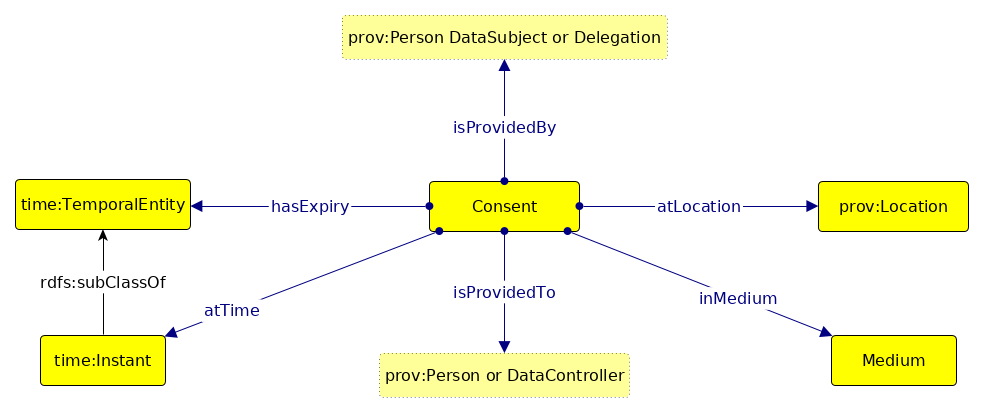
\includegraphics[width=0.8\linewidth]{img/gconsent_context.png}
    \caption{Concepts for representing context of consent in GConsent \cite{pandit_gconsent_2019}}
    \label{fig:vocabs:gconsent-context}
\end{figure}

\subsubsection{Consent States}
The state of consent determines the suitability of its usage as a legal basis in the processing of personal data.
From a compliance perspective, there are only two categories of states - one which permits legal processing of personal data, and the other being insufficient or prohibitive for  processing.
GConsent represents these using the concepts by sub-classing \texttt{Status} as \texttt{StatusValidForProcessing} and \texttt{StatusInvalidForProcessing} to indicate use of a consent instance as a valid or invalid legal basis as depicted in \autoref{fig:vocabs:gconsent-status}.
Instances provided to represent states of valid consent to indicate legal processing, and include - explicitly given, implicitly given, and given by delegation.
Instances provided that represent invalid states of consent to indicate processing should not be carried out include - unknown, not given, withdrawn, expired, invalidated, refused, and requested.

The use of state refers to tracking the consent of a data subject from the legal perspective, and is aimed to aid in the management of consent as an entity. For example, `unknown' reflects a situation where the status of consent is not known - which can occur when importing consent information data from another source.
This is distinct from `not given' which indicates an offer has been made for obtaining consent but the data subject has not yet provided any actionable response that could indicate acceptance or refusal - which are themselves represented by the states for `given' and `refused' respectively.
For meeting the obligations and requirements of GDPR compliance, it is not necessary to represent consent instances with states such as unknown or refused.
GConsent provides them based on the practical management of consent information where a Controller may wish to track the consent status of its processing operations throughout its life-cycle.
\begin{figure}[htbp]
    \centering
    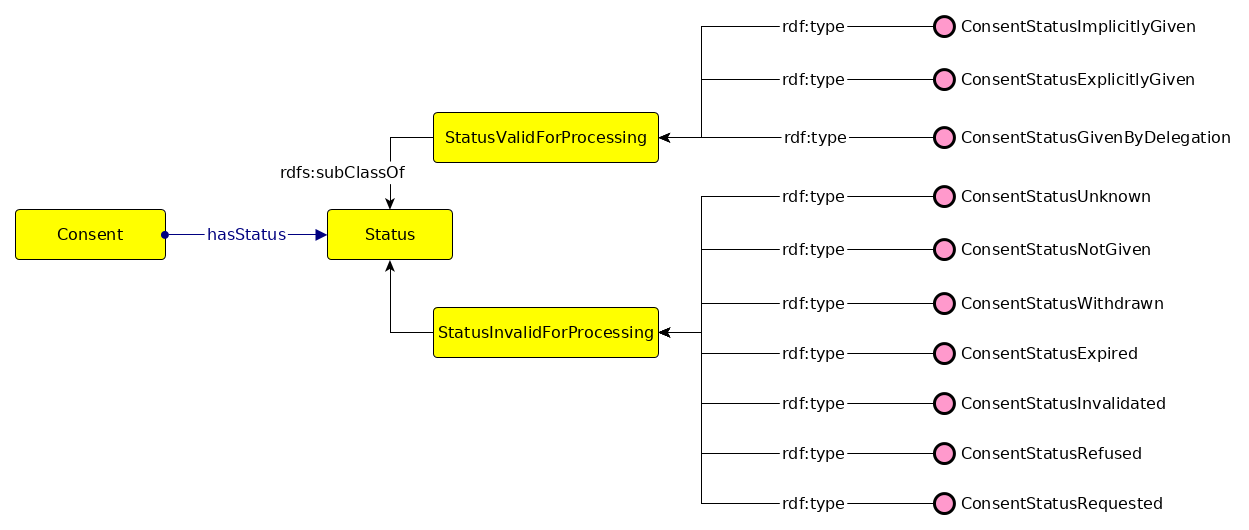
\includegraphics[width=\linewidth]{img/gconsent_status.png}
    \caption{Concepts representing state/status of consent in GConsent \cite{pandit_gconsent_2019}}
    \label{fig:vocabs:gconsent-status}
\end{figure}

GDPR requires keeping track of state change for consent. For example, when the status changes from given to withdrawn or when the state if changed to invalidated because of the choice of the controller or some legal requirement. Whenever a consent status changes, this results in a new consent instance being created, which also assists in capturing the context of the new consent (such as time instant). This leads to a chain of consent instances, where the `latest' consent is at the `end' of this chain and indicates the most recent operation regarding consent states. It is vital to record such provenance to demonstrate past processing was in compliance with the state of consent at that point in time and to show the changes in consent as part of its life-cycle.

\subsubsection{Example Use-Case}
The documentation of GConsent provides example applications of the ontology in four use-cases to demonstrate how information can be represented, which are - (i) change in consent state, (ii) capturing given consent, (iii) capturing consent given via delegation, and (iv) capturing consent when data is shared with a third party.
The fourth use-case is presented here to demonstrate the application of GConsent and the use of its concepts to represent information towards GDPR compliance.

The example, visually represented in \autoref{fig:vocabs:gconsent-example}, shows association of a third party in the role of a data processor\footnote{Under GDPR, a processor is not considered a third party, but has its own defined role as an entity associated with the Controller. However, from a lay person's perspective, the individual is the first party, the Controller is the second party, and any other entity is a third party. GConsent reflects this use in its structuring of entities where a Processor is considered a special type (sub-class) of Third Party.}
with whom the data is shared for the purpose of advertising. The association is captured by the instance \texttt{ex:AdvertisingArrangement} of type \texttt{prov:Association}, and has \texttt{ex:AdPartner} defined as a \texttt{gdprov:Processor} defined with the role as \texttt{gdprtext:Processor}. It is also possible to list out the specific arrangement for this association using the \texttt{prov:hadPlan} property and a \texttt{gdprov:Process} instance to list out the specific steps and entities involved in the data sharing arrangement.

The example serves to demonstrate the practical use of GConsent in representing information about consent, where PROV-O is used to specify relationships with a Processor. GConsent can be combined or supplemented by other ontologies to define such associations and practical reflections of data sharing agreements between parties. The defined instance of consent in the example enables a Controller to track the state of consent as the data subject is provided with the choice of whether to agree to this arrangement or to refuse it, and where upon agreement the option to exercise the right to modify and withdraw the consent is also provided.
\begin{figure}[htbp]
    \centering
    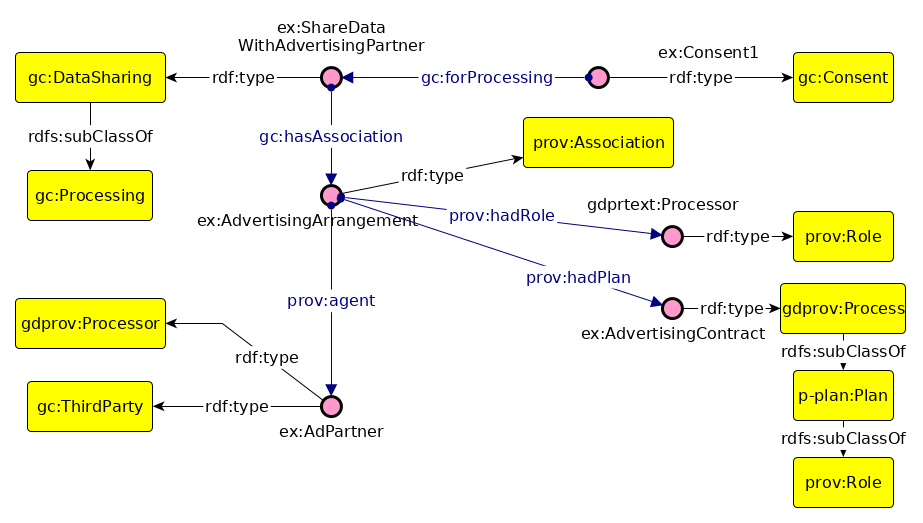
\includegraphics[width=0.8\linewidth]{img/gconsent_third_party_datasharing.png}
    \caption{GConsent representation of use-case involving third party data sharing \cite{pandit_gconsent_2019}}
    \label{fig:vocabs:gconsent-example}
\end{figure}

\subsection{Evaluation}\label{sec:voc:gconsent:evaluation}
GConsent as an ontology was evaluated regarding its capability to express information about consent using the methodology outlined in \autoref{sec:voc:methodology}.
This was an iterative process where the ontology was tested and modified to accommodate the requirements of the competency questions. Changes were made to the ontology where information was found to be missing or incorrectly modelled.
In particular, the iterations consisted of the degree and design of representing a dependency between purposes and processing operations associated with consent. These were ultimately rejected with the final iteration modelling purpose and processing independent of each other to provide greater granularity and reuse of these concepts.
GConsent was used and evaluated in the representation of consent information for a real-world website in the application of SHACL to validate information for GDPR compliance in \autoref{sec:testing:shacl}.

GConsent was published in the Extended Semantic Web Conference (ESWC) as a peer-reviewed publication \cite{pandit_gconsent_2019} in the Ontologies and Reasoning Track. As ESWC is a top-tier semantic web conference with a rigorous review process, the acceptance of GConsent demonstrates its contribution as a semantic web resource.
Along with this, the documentation of GConsent, available online, also provides extensive information about the ontology and its potential applications. It also provides a brief comparison of the ontology with relevant approaches within the state of the art.
GConsent, along with the Consent Receipt standard \cite{lizar_consent_2017}, had a direct impact on the design and development of consent information within the DPV. In particular, GConsent provided the concepts for expression of consent based on the GDPR and competency questions for integrating those with the rest of DPV.
Given the recency of the publication, GConsent does not currently have any citations (excluding self-citations).

\subsubsection{Fulfilment of Competency Questions}
The assessment of the extent to which GConsent provides concepts and relationships to answer the competency questions is presented in \autoref{table:gconsent:cq}. 
In these, the PROV-O and Time ontologies are used in conjunction with GConsent to represent provenance and temporal information about the consent and changes to it.
PROV-O is also used to capture the association and roles of entities in the activities associated with consent.
Based on these, GConsent satisfies the requirements of providing information for answering the compliance questions regarding consent and thus fulfils research objective $RO3(c)$.
\begin{table}[htbp]
\footnotesize
\centering
\rowcolors{1}{}{gray!10}
\begin{tabularx}{\textwidth}{|p{1cm}|X|p{4cm}|p{3.5cm}|}
\caption{Concepts and relationships in GConsent for answering competency questions} \\ \hline
\textbf{CQ} & \textbf{Question} & \textbf{Concepts} & \textbf{Properties} \\ \hline
\multicolumn{4}{|l|}{\textbf{Questions about consent}} \\ \hline
\textit{CMQ35} & Who is the consent about? & \textit{DataSubject} & \textit{isConsentForDataSubject} \\ \hline
\textit{CMQ36} & What type of Personal Data are associated with the Consent? & \textit{PersonalData} & \textit{forPersonalData} \\ \hline
\textit{CMQ37} & What type of Purposes are associated with the Consent? & \textit{Purpose} & \textit{forPurpose} \\ \hline
\textit{CMQ38} & What type of Processing are associated with the Consent? & \textit{Processing} & \textit{forProcessing} \\ \hline
\textit{CMQ39} & What is the Status of Consent? & \textit{Status} & \textit{hasStatus} \\ \hline
\textit{CMQ87} & Is the current status valid for processing? & \textit{StatusValidForProcessing, StatusInvalidForProcessing} & \textit{hasStatus} \\ \hline
\textit{CMQ46} & Who is the consent given to? & \textit{prov:Person, DataController} & \textit{isProvidedTo} \\ \hline
\multicolumn{4}{|l|}{\textbf{Questions about how the consent was created/given/acquired/changed/invalidated}} \\ \hline
\textit{CMQ42, CMQ76} & Who created/gave/acquired/invalidated the consent? & \textit{DataSubject, Delegation} & \textit{isProvidedBy} \\ \hline
\textit{CMQ41, CMQ77} & If consent was created/gave/acquired/invalidated through Delegation, who acted as the Delegate? & \textit{prov:Person, Delegation} & \textit{prov:agent} \\ \hline
\textit{CMQ43} & If consent was created/gave/acquired/invalidated through Delegation, what was the role played by Delegate? & \textit{prov:Role} & \textit{prov:hadRole} \\ \hline
\textit{CMQ44} & If consent was created/gave/acquired/invalidated through Delegation, how was the delegation executed? & \textit{prov:Activity} & \textit{prov:hadActivity} \\ \hline
\multicolumn{4}{|l|}{\textbf{Questions about the context of how consent was created/gave/acquired/invalidated}} \\ \hline
\textit{CMQ53, CMQ84} & What is the location of associated with consent? & \textit{prov:Location} & \textit{atLocation} \\ \hline
\textit{CMQ54, CMQ85} & What is the medium associated with consent? & \textit{Medium} & \textit{inMedium} \\ \hline
\textit{CMQ55, CMQ86} & What is the timestamp associated with the consent? & \textit{time:Instant} & \textit{atTime} \\ \hline
\textit{CMQ56, CMQ87} & What is the expiry of the consent? & \textit{time:TemporalEntity} & \textit{hasExpiry} \\ \hline
\textit{CMQ82} & What artefacts were shown when consent was acquired/changed/created/invalidated? & \textit{prov:Entity} & \textit{prov:used} \\ \hline
\multicolumn{4}{|l|}{\textbf{Questions related to Third Party associated with the consent}} \\ \hline
\textit{CMQ57} & Is the purpose or processing associated with a third party? & \textit{prov:Association}, \textit{ThirdParty} & \textit{hasAssociation, prov:agent} \\ \hline
CMQ58 & What is the role played by the third party in the purpose or processing? & Role & prov:hadRole \\ \hline
\end{tabularx}
\label{table:gconsent:cq}
\end{table}

\subsubsection{Comparison with SotA}
The existing approaches regarding consent were presented and analysed in \autoref{sota:analysis:consent}, with the observation about the lack of approaches modelling consent as required for GDPR compliance.
\autoref{table:gconsent:sota} demonstrates a comparison of GConsent with the SotA based on the attributes used in this analysis.
The column headings indicate the representation of information within an approach and are abbreviated to indicate - Personal Data (PD), Purpose (Pu), Processing (Pr), Data Sharing (Sh), Data Storage (St), Recipients (Rp), Data Source (S), Withdrawal of consent (W), Delegation (D), Visualisation (V), Significant effects of processing (SE), (Ct): Context (Ct), Types or States (T).
A check mark (\cmark) indicates the approach provides or models that information category, and a blank cell indicates that the approach does not provide representation for that information or that there is no open and public information available regarding its provision.
\begin{table}[htbp]
\footnotesize
\centering
\caption{Representation of consent in SotA}\label{table:gconsent:sota}
\rowcolors{1}{}{gray!10}
\begin{tabularx}{\textwidth}{|l|X|X|X|X|X|X|X|X|X|X|X|X|}
\hline

\textbf{Work} & \textbf{PD} & \textbf{Pu} & \textbf{Pr} & \textbf{Sh} & \textbf{St} & \textbf{Rp} & \textbf{S} & \textbf{W} & \textbf{D} & \textbf{SE} & \textbf{Ct} & \textbf{T} \\ \hline
\rowcolor[gray]{0.8}
GConsent & \cmark & \cmark & \cmark & \cmark & \cmark & \cmark & \cmark & \cmark & \cmark & \cmark & \cmark & \cmark \\ \hline
SPECIAL & \cmark & \cmark & \cmark & \cmark & \cmark & \cmark &  & \cmark &  &  &  &  \\ \hline
SPL+CitySPIN & \cmark & \cmark & \cmark & \cmark & \cmark & \cmark &  & \cmark &  &  &  &  \\ \hline
Lodge et al & \cmark & \cmark &  &  &  &  &  &  &  &  &  &  \\ \hline
Peras & \cmark & \cmark & \cmark & \cmark & \cmark &  &  & \cmark &  &  &  &  \\ \hline
Coletti et al & \cmark & \cmark &  &  &  &  & \cmark & \cmark &  &  &  &  \\ \hline
AdvoCATE & \cmark & \cmark &  &  & \cmark & \cmark &  &  &  & \cmark & \cmark &  \\ \hline
RestAssured & \cmark & \cmark & \cmark & \cmark & \cmark & \cmark &  &  &  &  &  &  \\ \hline
OPERANDO & \cmark & \cmark & \cmark & \cmark &  & \cmark &  &  &  &  &  &  \\ \hline
PoSEID-on & \cmark &  &  &  &  & \cmark &  &  &  &  &  &  \\ \hline
MHMD & \cmark &  &  &  &  &  &  &  &  &  &  &  \\ \hline
DECODE & \cmark & \cmark &  &  & \cmark &  &  &  &  &  &  &  \\ \hline
Consent Receipt & \cmark & \cmark &  &  &  &  &  &  &  &  & \cmark & \cmark \\ \hline

\end{tabularx}
\end{table}

The table demonstrates the contribution of GConsent to the state of the art. 
Compared to the SotA, GConsent provides novel contributions for the representation of consent for GDPR compliance and thus extends the state of the art.
In particular, the depiction of delegation is more detailed and provides representation of information based on compliance requirements of GDPR.
As the table depicts, GConsent is currently the only approach that models delegation based on its potential relevancy to the evaluation of GDPR compliance.
GConsent is also novel in the provision of consent states which enable documenting of information from a controller's perspective regarding the evolution of consent throughout its life-cycle. This is useful for the management of consent as an entity in an information management system such as a database.
The SotA usually limits the consent state to given or withdrawn without consideration to its other states within the life-cycle as an entity.

\subsubsection{Application to external use-case from SPECIAL project}\label{sec:gconsent:use-case:SPECIAL}
The use-case described in \autoref{sec:gdprov:use-case:SPECIAL} is used here to demonstrate the use and sufficiency of GConsent in management of consent information. The use-case concerns the scenario where a data subject named Sue gives consent to BeFit company for sharing her activity profile with other companies for receiving targeted ads. She later receives ads from a local Gym and investigates to find that the Gym is using her activity profile shared by BeFit - and that this activity is consistent with her previously given consent. She then withdraws her consent and asks both companies to delete her data.

The representation of this use-case using GConsent consists of using its concepts to represent the information, and to then utilise SPARQL to answer the queries - similar to the exercise in \autoref{sec:gdprov:use-case:SPECIAL} for GDPRov. \autoref{table:gconsent:use-case:SPECIAL} presents the concepts for representing the use-case using GConsent, GDPRov, and SPECIAL vocabularies. The corresponding RDF representation using GConsent is provided in \autoref{code:gconsent:use-case:special} with the queries for deriving answers to questions (i) - (iv) in the use-case are provided in \autoref{code:gconsent:use-case:special-sparql}.
\begin{center}
\scriptsize
\begin{tabularx}{\textwidth}{|p{0.3\linewidth}|X|X|X|}
\caption{GConsent concepts to represent external use-case from SPECIAL}\label{table:gconsent:use-case:SPECIAL} \\
\toprule
\textbf{Statement} & \textbf{GConsent} & \textbf{GDPRov} & \textbf{SPECIAL} \\
\midrule
\endhead
Sue & \texttt{DataSubject} & \texttt{DataSubject} & \texttt{DataSubject} \\ \hline
BeFit & \texttt{DataController} & \texttt{DataController} & \texttt{Controller} \\ \hline
Biomedical parameters, heart rate, calories consumption, activity profile & \texttt{PersonalData} & \texttt{PersonalData} & \texttt{Data} \\ \hline
Collect data & \texttt{Collection Of PersonalData} & \texttt{Data Collection Activity} & \texttt{Collect} \\ \hline
Provide feedback on activity & \texttt{Purpose} & \texttt{Purpose} & \texttt{Purpose} \\ \hline
Give consent (opt-in) & N/A & \texttt{Acquire Consent Activity} & \texttt{ConsentAssertion} \\ \hline
Targeted ads related to fitness & \texttt{Purpose} & \texttt{Purpose} & \texttt{Purpose} \\ \hline
Share data & \texttt{Sharing Of Personal Data} & \texttt{Data Sharing Activity} & \texttt{Recipient} \\ \hline
Gym & \texttt{ThirdParty} & \texttt{ThirdParty} & \texttt{Recipient} \\ \hline
Consent agreement & \texttt{Consent Status Explicitly Given} & \texttt{GivenConsent} & \texttt{LogEntryContent} \\ \hline
Delete data & \texttt{Deletion Of Personal Data} & \texttt{Data Deletion Activity} & N/A \\ \hline
Withdraw consent & N/A & \texttt{Withdraw Consent Activity} & \texttt{ConsentRevocation} \\ \hline
Withdrawn consent & \texttt{Consent Status Withdrawn} & N/A & N/A \\
\bottomrule
\end{tabularx}
\end{center}
\begin{listing}[htbp]
\begin{minted}{turtle}
# Entities
:Sue a gc:DataSubject .
:BeFit a gc:DataController .
:Gym a gc:ThirdParty .
# Personal Data
:Activity_Profile a gc:PersonalData .
# Purpose
:Targeted_ads_related_to_fitness a gc:Purpose .

# Sue gives consent to BeFit
:Consent1_registration a gc:Consent ;
	gc:isConsentForDataSubject :Sue ;
	gc:isProvidedToController :BeFit ;
	gc:forPurpose :Targeted_ads_related_to_fitness ;
	gc:forProcessing gc:CollectionOfPersonalData, 
		gc:ShareDataForTargetedAds ;
	gc:forPersonalData :Activity_Profile ;
	gc:hasStatus gc:ConsentStatusExplicitlyGiven .

# BeFit shares data with Gym 
# assumed similar 'policy' structure as SPECIAL
:ShareDataForTargetedAds a gc:DataSharing ;
	gc:involvesThirdParty :Gym .
	gc:sharesDataWithThirdParty :Gym .

:Consent_info_shared_by_BeFit_with_Gym a gc:Consent ;
	gc:isConsentForDataSubject :Sue ;
	gc:isProvidedTo :BeFit ;
	gc:forPurpose :Targeted_ads_related_to_fitness ;
	gc:forProcessing gc:UseOfPersonalData ;
	gc:forPersonalData :Activity_Profile ;
	gc:hasStatus gc:ConsentStatusExplicitlyGiven .	

# Sue withdraws consent
:Consent2_withdraw a gc:Consent ;
	gc:isUpdatedConsentFor :Consent1_registration ;
	gc:forPurpose :Targeted_ads_related_to_fitness ;
	gc:forProcessing gc:CollectionOfPersonalData, 
		gc:ShareDataForTargetedAds ;
	gc:forPersonalData :Activity_Profile ;
	gc:hasStatus gc:ConsentStatusWithdrawn .

\end{minted}
\caption{GConsent representation of external use-case from SPECIAL}
\label{code:gconsent:use-case:special}
\end{listing}
\begin{listing}[htbp]
\begin{minted}{sparql}
# Query (i)
# retrieves :Activity_Profile as data shared for Sue
# queried over Gym's records
SELECT ?personal_data
WHERE {
	?_ gc:isConsentForDataSubject :Sue .
	?_ gc:forPersonalData ?personalData .
}

# Query (ii)
# retrieves :BeFit as data source
# retrieves :Targeted_ads_related_to_fitness as purpose
# queried over Gym's records
SELECT ?party, ?purpose {
	?_ gc:isConsentForDataSubject :Sue .
	?_ gc:forPersonalData :Activity_Profile .
	?_ gc:isProvidedTo ?party .
	?_ gc:forPurpose ?purpose .
}

# Query (iii)
# retrieves :CollectionOfPersonalData as the processing operation
# from which it needs to be inferred that data is collected from Sue
# queried over BeFit's records
SELECT ?data_processing {
    ?_ gc:forPersonalData :Activity_Profile .
    ?_ gc:forProcessing ?data_processing .
}

# Query (iv)
# retrieves :Consent1_registration as satisfying
# conditions for data sharing with Gym
# queried over BeFit's records
SELECT ?consent
WHERE {
	?consent a gc:Consent .
	?consent gc:isConsentForDataSubject :Sue .
	?consent gc:forPersonalData :Activity_Profile .
	?consent (gc:forProcessing/gc:sharesDataWithThirdParty) :Gym .
}


\end{minted}
\caption{SPARQL queries using GConsent for external use-case from SPECIAL}
\label{code:gconsent:use-case:special-sparql}
\end{listing}

From the above representation and queries, the use of GConsent demonstrates the use of terms (purpose, sharing, etc.) closer to those of SPECIAL as compared to GDPRov's representation in \autoref{sec:gdprov:use-case:SPECIAL}.
At the same time, the inability to represent information about activities such as how the data was collected or shared is also evident since GConsent does not represent them while GDPRov does.
From a consent perspective, the consent `records' represented using GConsent are more clear and concise in terms of what the consent related to, and how it was withdrawn.
The above representation therefore demonstrates GConsent's use in managing consent information, with the SPARQL queries used to retrieve the answers to questions pertaining to use of Sue's personal data within the use-case.

\subsection*{Summary}
GConsent is an ontology for the representation of consent and its associated information for GDPR compliance. It fulfils the research objective $RO3(c)$ and along with GDPRov forms the second major contribution of this thesis.
GConsent has been published in a peer-reviewed publication and is available online as an open and reusable resource along with an extensive and descriptive documentation.

GConsent is currently the only approach within the state of the art to provide representations of attributes of consent and its states based on the requirements of the GDPR.
GConsent thus represents a novel representation of consent based on GDPR and provides the concept of states for practical management of consent information from a controller's perspective. It also provide detailed information representation regarding the context of consent which enables documenting information required for evaluating the validity of consent under GDPR compliance requirements.

% DPV
\section{Data Privacy Vocabulary (DPV)}\label{sec:voc:DPV}
The Data Protection Vocabulary \cite{pandit_creating_2019} is a semantic web ontology for representing information about personal data handling based on legal requirements such as those for GDPR compliance.
It is the outcome of work done by the W3C Data Privacy Vocabularies and Controls Community Group (DPVCG) which consists of collaboration between a community of academics, researchers, industry stakeholders, and legal experts as initially described in \autoref{sec:intro:dpvcg}.
The DPVCG aims to work towards establishment of interoperable standards regarding representing information about personal data processing for which there are currently no existing standards.

The DPVCG was initiated as an outcome of the SPECIAL project \cite{pandit_d6.5_2019}, and therefore bears close association and alignment with the SPECIAL vocabularies.
In particular, the SPECIAL core vocabulary was used as the basis to create the DPV core vocabulary, providing compatibility between the DPV and SPECIAL vocabularies and frameworks.

The DPV reflects a community consensus in its representation of information regarding data protection and personal data processing. While being a generic vocabulary, much of its design is based on and reflected by the requirements of the GDPR. The DPV, and by extension the DPVCG, reflect an ongoing effort to provide practical and useful semantic representations of information in an open and interoperable machine-readable form. 

\subsection{Relevance of DPV to this thesis}
The ontologies presented in this thesis as research contributions - namely GDPRtEXT, GDPRov, and GConsent - were part of the state of the art analysed by DPVCG in its methodology \cite{pandit_creating_2019}.
In addition, by being an active member of the DPVCG and a contributor in the creation of DPV, the author of this thesis has applied the experience of developing presented research to influence the design and modelling of information within the DPVCG.

The publication presenting DPV \cite{pandit_creating_2019} presents its creation methodology and concepts where the author of this thesis was a co-first author.
In addition to these, the vocabulary specification published online lists the author of this thesis as an co-editor and author of the ontology.
The deliverable D6.5 \cite{pandit_d6.5_2019} of the SPECIAL project presents the work of the DPVCG by describing the DPV based on the peer-reviewed publication of DPV \cite{pandit_creating_2019} and also features the author of this thesis as one of the lead authors within the deliverable.

Owing to the involvement of the author and the overlap between DPV and the research question and developed ontologies, the DPV is a research contribution influenced by the research presented in this thesis.
This section describes the DPV and compares it with the ontologies presented in this thesis to provide an extent of their overlap and provide the basis for comparison.
It demonstrates the differences in representation of information, scope, and methodology and their complimentary nature in representing information for GDPR compliance.

\subsection{Overview of DPV}
\subsubsection{Description of Data Privacy Vocabulary}
The DPV ontology is published at the W3C namespace \url{http://w3.org/ns/dpv} with its documentation and uses the namespace prefix \texttt{dpv}. 
The current iteration of vocabulary provides classes and properties to annotate and categorise information about legally compliant personal data handling. In this context, personal data handling refers to all operations associated with processing of personal data and its management including organisational measures which indirectly affect processing.

The DPV is a pseudo-modular ontology with a set of core concepts referred to as the `\textit{Base Ontology}' and modular extensions further expanding each concept in the form of a taxonomy. The base ontology represents the top-level classes for defining a policy of legal personal data handling.
The core concepts, visualised in \autoref{fig:vocabs:dpv-core}, consist of personal data category, processing, purpose, legal basis, data controller, recipient, data subject, technical and organisational measures, and the top-level concept of personal data handling which ties them together.

\begin{figure}[htbp]
    \centering
    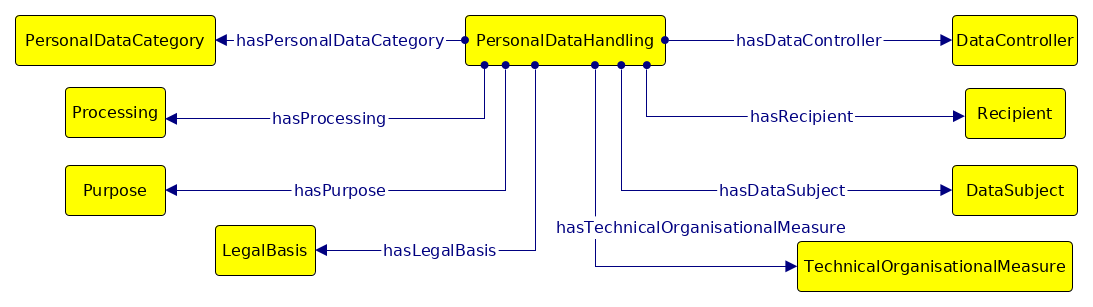
\includegraphics[width=\linewidth]{img/dpv-personaldatahandling.png}
    \caption{Core concepts in DPV \cite{pandit_creating_2019}}
    \label{fig:vocabs:dpv-core}
\end{figure}

\subsubsection{Personal Data Categories}
DPV uses the taxonomy provided by EnterPrivacy\footnote{\url{https://enterprivacy.com/wp-content/uploads/2018/09/Categories-of-Personal-Information.pdf}} to define a broad hierarchy of personal data categories based on the nature of information (financial, social, tracking) and to its inherent source (internal, external). 
In addition to these, the class \texttt{dpv:Special\-Category\-Of\-PersonalData} represents categories that are `special' or `sensitive' based on GDPR’s Article 9.

These personal data categories can be further extended by using the sub-class mechanism to depict specialised concepts such as `likes regarding movies'.
Sub-classing also enables representation of specific contexts such as derivation of personal data as represented by the class \texttt{dpv:DerivedPersonalData}.
This is useful to represent practical representation of personal data categories such as inference of opinions from social media.
Similar classes can be additionally added to specify contexts such as use of machine learning, accuracy, and source.
The aim of the providing such high-level concepts is to provide a sufficient coverage of abstract categories of personal data which can be extended using the subclass mechanism to represent concepts used in the real-world. 

\subsubsection{Purposes}
Purposes in DPV are organised hierarchically by using the sub-class mechanism to represent high-level and generic purposes of data handling.
Purposes provided in DPV include service provision, R\&D, commercial interest, security, service optimisation, and service personalisation. These are further extended to provide a total of 31 generic purposes.
These may be extended by further sub-classing to create more specific purposes as applicable to a scenario.
As GDPR requires a specific purpose to be declared in an understandable manner, specific purposes can be created using sub-classes of one or several \texttt{dpv:Purpose} categories to make them as specific to the use-case as possible.
 Purposes can be restricted to specific \texttt{contexts} using the class \texttt{dpv:Context} and the property \texttt{dpv:hasContext}.
Purposes can also be restricted to a specific \texttt{business sector} using the class \texttt{dpv:Sector} and the property \texttt{dpv:hasSector}.

\subsubsection{Processing Categories}
DPV provides a hierarchy of processing categories based on the requirements of regulations such as GDPR. 
DPV defines top-level classes to represent the following broad categories of processing - Disclose, Copy, Obtain, Remove, Store, Transfer, Transform, and Use.
Each of these are then again further expanded using sub-classes to provide 33 processing categories, which includes terms defined in the definition of processing in GDPR (Article 4-2).
The DPV provides properties with a boolean range to indicate the nature of processing regarding \texttt{Systematic Monitoring}, \texttt{Evaluation or Scoring}, \texttt{Automated Decision-Making}, \texttt{Matching or Combining}, \texttt{Large Scale processing}, and \texttt{Innovative use of new solutions} - as these affect assessment of legal data processing under GDPR.

\subsubsection{Technical and Organisational Measures}
GDPR Article 32 requires implementing appropriate measures by taking into account the state of the art, the costs of implementation and the nature, scope, context and purposes of processing, as well as risks, rights and freedoms.
These are represented as technical and organisational measures in the DPV.
Examples include pseudo-anonymisation and encryption of personal data, the ability to restore the availability and access to personal data in a timely manner in the event of a physical or technical incident, and a process for regularly testing, assessing and evaluating the effectiveness of technical and organisational measures for ensuring the security of the processing.
The generic property \texttt{dpv:measureImplementedBy} enables referencing the implementation measure as a comment or IRI.
The class \texttt{StorageRestriction} provides expression of measures used for storage of data with two specific properties provided for storage location and duration restrictions.

\subsubsection{Consent and Legal Bases}
DPV provides \texttt{dpv:LegalBasis} as a top-level concept to represent various legal bases that can be used for justifying processing of personal data.
The definition of a `legal basis' is based on the justification for processing which has a provision in the law. The concept itself is not based on any specific jurisdiction, but needs to be interpreted in terms of the legal bases defined and provided within the laws applicable within a jurisdiction.

For the GDPR, which is a EU specific law, and therefore is not binding in the interpretation of legal bases across all use-cases, the DPV provides the legal bases specific to GDPR as a separate aligned vocabulary under the \url{https://www.w3.org/ns/dpv-gdpr} and namespace (prefix: \texttt{dpv-gdpr}). 
This vocabulary defines the legal bases defined by Articles 6 and 9 of the GDPR to represent the legal justification of processing personal data.

Consent as a special case of legal basis provided by the GDPR is provided with additional properties and classes within the core DPV vocabulary to reflect the information requirements associated with its validity as a legal basis.
The concepts associated with consent provide terms to describe consent provision, withdrawal, and expiry.
The structure of these was adapted from an analysis of existing work in the form of Consent Receipt \cite{lizar_consent_2017} and GConsent \cite{pandit_gconsent_2019} with the intention to enable documenting attributes associated with consent which can demonstrate and evaluate its validity based on requirements of the GDPR.

\subsection{Comparing DPV with GDPRtEXT, GDPRov, and GConsent}
DPV has several commonalities with the ontologies presented in this thesis arising from the common aim of representing information for legal compliance with laws such as the GDPR.
However, the aim and granularity of representing information about all attributes relevant to the processing of personal data differentiates the DPV from the specific focus of ontologies presented in this thesis.
Given the high-level and abstract nature of DPV in its concepts, and the more granular and representative focus of developed ontologies, there is a possibility of aligning or combining the two.
While there have been no efforts to carry out an exercise to combine or align the developed ontologies with DPV, their comparison as presented here demonstrates the possibility and applicability of such an approach.

\subsubsection{Representing information about GDPR concepts}
GDPRtEXT provides a linked data version of GDPR and a SKOS glossary of concepts associated with GDPR compliance, which can be used to link information to the clauses and concepts of GDPR.
This has been used by GDPRov and GConsent to define the source of its concepts within the text of GDPR.

The DPV, whose concepts represent a generic legal term, does not link its concepts to the GDPR except in cases where the defined concept was directly taken from the definition provided by GDPR.
In such cases, it uses the URI format prescribed by the EU Publications Office to indicate the specific clause of GDPR. The URI format\footnote{The format is based on using templates to indicate the alphanumeric characters of articles and clauses. The template format can be represented as: \texttt{https://eur-lex.europa.eu/eli/reg/\{year\}/\{number\}/art\_\{X\}/par\_\{X\}/pnt\_\{X\}/oj}}, similar in its structuring of contents with GDPRtEXT, is based on an upcoming iteration\footnote{The information is based on a private communication between the author of the thesis with members of the EU Publications Office. The prescribed IRI, while not officially published or documented, currently resolves to the web-page of the legislation, which in this case is the GDPR.} of the ELI vocabulary which will be used in all EU published legislations to offer granular linking to their clauses.
Since the format prescribed by EU Publications Office is authoritative in its nature, the links provided by GDPRtEXT need to be aligned or replaced with those defined using the newer ELI format which offers further advantages in provision of concepts and granularity.

One of the aims of the DPVCG is to provide a glossary of concepts associated with legal personal data handling. For this, the concepts of DPV itself can be considered as a glossary of terms, though not defined as such within the ontology. This use of `glossary' refers to providing the concepts to an adopter in order to represent the required information. Since these terms do not necessarily arise from a particular legislation, their sources are based more on their use as a commonly understood concept or notion within the legal domain.
In terms of coverage, GDPRtEXT focuses more on terms directly obtained through the text of the GDPR while the DPV focuses on the modelling of concepts based on their relevance to defining personal data handling.
Therefore, while there is a small overlap in the concepts directly associated with GDPR, the two vocabularies differ in their provision of terms. To further exemplify this distinction, the DPV aims to offer terms that reflect real-world practices while GDPRtEXT focuses on the legal text of GDPR. This is evident from the hierarchical taxonomy of concepts in DPV, such as for personal data categories and purposes.

\subsubsection{Representing information about activities}
The DPV does not provide representation of activities through which it can be compared with GDPRov.
Instead, DPV provides concepts to represent `processes' taking place within an organisation, such as those for ensuring technical and organisational measures, purposes, and processing.
The modelling of an instance of personal data handling, which consists of specifying the purpose, processing, and technical \& organisational measures, can be compared with the modelling of plans in GDPRov where a purpose represents a plan and its steps represent processing activities - which can be further annotated with measures and legal bases.
Through this, it can be summarised that the focus of GDPRov is on representing the activities with arbitrary granularity, and that of DPV on providing metadata about the processing without dealing with the underlying details of implementation. With this, it is possible to define an instance of personal data processing using DPV to indicate the high-level summary of associated information and further expand it using GDPRov to represent details of processes and capture their provenance in ex-ante/ex-post phases.

\subsubsection{Representing information about consent}
The DPV and GConsent both provide concepts to represent information about consent based on the requirements specified by GDPR.
In this, both share the aim to document the context of consent with a view towards establishing its validity and compliance.
The difference between the two is based on the granularity and use of existing vocabularies to represent this information.

The DPV utilises the model provided by its core or base vocabulary to represent information by specifying consent as the legal base used to justify processing of personal data.
In addition to this, it provides properties to indicate the specific notice displayed to obtain consent, its expiry, the obtaining or provision of consent, and its withdrawal.
In this, attributes such as timestamp, method used to carry out the provision and withdrawal are used to indicate information regarding how the consent was obtained.
This is based on notion of providing a form of the Consent Receipt based on requirements of the GDPR.

The DPV does not prescribe or utilise any existing vocabulary to specify information.
In contrast, GConsent provides similar concepts as the DPV base vocabulary and uses vocabularies of PROV-O and GDPRov to represent the information about activities.
Given that GConsent was an input to the DPV and by extension influential in its modelling of consent, there is a degree of compatibility between the two based on the similarity of concepts.
In this, GConsent is a more detailed vocabulary while DPV provides a minimal set of concepts regarding consent but is more expressive in representing the overall information regarding data processing.

\subsection{Comparing DPV with SotA}\label{sec:voc:dpv-sota}
This sections compares the DPV with approaches presented in the SotA in \autoref{chapter:sota}.
The aim of this exercise to demonstrate the extent of DPV's contributions and presents its relation with the rest of approaches in SotA.
Since the DPV is not presented as a direct contribution of this thesis, its evaluation is not within the scope of this thesis.

The aim of the DPV as established by the DPVCG is providing a vocabulary for personal data handling which concerns representation of information relevant for legal compliance - in this case associated with GDPR. Based on this, the DPV is a vocabulary useful towards representing the state of processing rather than a framework or methodology that can be used to evaluate compliance.
Currently, the DPV is not accompanied by any documentation demonstrating its use or application in use-cases, with such activities planned in the future.

Comparing the DPV with other vocabularies in the SotA, the DPV provides a large amount of concepts as a top-down modelled taxonomy which can be expanded with additional concepts. This enables it to be adapted and expanded within any use-case, while the drawbacks of this are that it cannot be readily used in its current state.
This aspect of the DPV is novel within the SotA as no other approach aims to provide a similar taxonomy of concepts, and does not incorporate the requirements of extending it for a given use-case such as through the sub-classing mechanism.

The DPV base vocabulary provides a compact structure representing personal data handling which aims to represent all the relevant information required to evaluate and demonstrate compliance.
In this, it bears resemblance to the SPECIAL core vocabulary \cite{bonatti_special_2018-2} given that the DPVCG was an extension of SPECIAL's work on its vocabularies.
This approach is more suitable for representation or documentation of information from a compliance perspective, and is not intended to be specific to any particular law - though the GDPR clearly has a significant influence on the vocabulary.
This is again in contrast to the approaches in SotA which are often intended to be applied to a particular legislation and a specific use-case.

The representation of technical and organisational measures is the most distinctive feature of DPV, as currently no other approach within the SotA provides concepts to represent these.
While there have been efforts to establish vocabularies regarding specification and representation of privacy policies, these tend to focus on the use of concepts such as purpose, processing, data storage, data sharing, third parties - which have been utilised quite commonly in SotA.

\section*{Chapter Summary}
The chapter presented the ontologies created to fulfil the research objective $RO3$ along with the methodology used for their development and their evaluation. It also provides a comparison of the ontologies with related approaches of the SotA presented in \autoref{chapter:sota}.

The ontology engineering process was presented in \autoref{sec:intro:ontology-engineering} and described the methodology used for creating ontologies based on best-practices and guidelines advocated by the community. This included ensuring ontology quality, documentation, and releasing developed resources under an open and permissive license.
It also described utilisation of compliance questions presented in \autoref{sec:info:compliance-questions} as competency questions.

The presented ontologies consisted of GDPRtEXT, GDPRov, and GConsent.
GDPRtEXT, presented in \autoref{sec:voc:GDPRtEXT}, provides a linked data version of the text of GDPR created by extending the official ELI \cite{ELI_2012} ontology to represent its granular clauses. It also presents a SKOS glossary of concepts associated with GDPR compliance. GDPRtEXT enables the association and linking of information with the concepts and text of GDPR through the use of persistent IRIs. It thus fulfils research objective $RO3(a)$. GDPRtEXT extends the state of the art by providing an ELI-compatible extension capable of representing GDPR clauses at a granular level. It is also novel in providing a thesauri of concepts associated with GDPR compliance.

GDPRov provides an OWL2 ontology for representing activities associated with personal data and consent in ex-ante and ex-post phases. It is presented in \autoref{sec:voc:GDPRov}.
The ontology is based on extending the existing ontologies of PROV-O \cite{lebo_prov-o_2013} and P-Plan \cite{garijo_p-plan_2014} with GDPR terminology using GDPRtEXT to represent activities in context of compliance requirements. GDPRov is novel in the use of PROV-O and P-Plan together based on the scientific workflow model to represent processes for GDPR compliance.
It provides an extensible model that can be used for representing processes related to compliance and can be extended for other purposes as well.
The use of GDPRov enables capturing the provenance of plans or snapshots of a system at a given time and document them as evidence of planned and maintained compliance.
The use of P-Plan with PROV-O enables associating execution of activities with their intended planning and thereby provides systematic linking of ex-ante and ex-post compliance information.
GDPRov thus fulfils the research objective $RO3(b)$.

The representation of consent is provided by GConsent - an OWL2 ontology presented in \autoref{sec:voc:GConsent} that fulfils research objective $RO3(c)$.
GConsent provides representation of information relevant for evaluation of consent under GDPR obligations and requirements.
It extends on the notion of consent as an provenance entity in GDPRov and models the life-cycle of consent based on the concept of states.
State or status of consent reflects its suitability for use as a legal basis for processing and is modelled based on the management of consent information from an organisation's perspective. In this GConsent is novel within the SotA.
GConsent is also novel in the provision of concepts related to consent for the GDPR as it provides the most verbose vocabulary for representing information regarding consent.

The chapter also presented the DPV vocabulary published by the W3C Data Privacy and Vocabularies Community Group (DPVCG). The author of the thesis was an active contributor to the DPV, and subsequently the DPV shares its aim and bears similarity to the research presented in this thesis. \autoref{sec:voc:DPV} provides a summary of the DPV and compares it with the ontologies presented as contributions in this thesis, namely GDPRtEXT, GDPRov, and GConsent. A comparison of DPV with the SotA is also provided.
The DPV is intended to provide a vocabulary for representing information about personal data handling, and is not limited to the GDPR though it is influenced by it. It reflects a community consensus and is intended to be standardised, thereby providing a basis for its adoption.

Through these developed ontologies and the significance of the DPV, the primary problem guiding this research and outlined in the beginning of this thesis (\autoref{sec:intro:background}) of representing information and associating it with the GDPR has been addressed.
In the next chapter, the use of semantic web technologies to query this information to answer the compliance questions, such as those presented in \autoref{sec:info:compliance-questions}, is presented. The chapter also presents the use of semantic web technologies in validating information to ensure its correctness for assessing GDPR compliance based on constraints presented in \autoref{sec:info:constraints}.
The querying and validation of information are presented as minor contributions of the thesis, and satisfy the research objectives $RO4$ and $RO5$.
They utilise real-world use-cases to demonstrate application of the developed ontologies of GDPRtEXT, GDPRov, and GConsent to represent, query, and validate information for GDPR compliance.
